%%%%%%%%%%%%%%%%%%%%%%%%%%%%%%%%%%%%%%%%%%%%%%%%%%%%%%%%%%%%%%%%%%%%%%%%%%%%%%%%
%2345678901234567890123456789012345678901234567890123456789012345678901234567890
%        1         2         3         4         5         6         7         8

\documentclass[letterpaper, 10 pt, conference]{ieeeconf}  % Comment this line out if you need a4paper

%\documentclass[a4paper, 10pt, conference]{ieeeconf}      % Use this line for a4 paper

\IEEEoverridecommandlockouts                              % This command is only needed if 
                                                          % you want to use the \thanks command

\overrideIEEEmargins                                      % Needed to meet printer requirements.

%In case you encounter the following error:
%Error 1010 The PDF file may be corrupt (unable to open PDF file) OR
%Error 1000 An error occurred while parsing a contents stream. Unable to analyze the PDF file.
%This is a known problem with pdfLaTeX conversion filter. The file cannot be opened with acrobat reader
%Please use one of the alternatives below to circumvent this error by uncommenting one or the other
%\pdfobjcompresslevel=0
%\pdfminorversion=4

% See the \addtolength command later in the file to balance the column lengths
% on the last page of the document

% The following packages can be found on http:\\www.ctan.org
\usepackage{graphics} % for pdf, bitmapped graphics files
\usepackage{epsfig} % for postscript graphics files
\usepackage{mathptmx} % assumes new font selection scheme installed
\usepackage{times} % assumes new font selection scheme installed
\usepackage{amsmath} % assumes amsmath package installed
\usepackage{amssymb}  % assumes amsmath package installed

\usepackage{algorithm}
\usepackage{algorithmic}
\usepackage{bm} % in the preamble


\usepackage{cite}
\usepackage{amsmath,amssymb,amsfonts}
\usepackage{algorithmic}
\usepackage{graphicx}
\usepackage{textcomp}
\usepackage{xcolor}
\definecolor{lightblue}{RGB}{30,144,255}
\usepackage[hidelinks]{hyperref}
\hypersetup{
    colorlinks=true,
    linkcolor=lightblue,
    citecolor=lightblue,
    urlcolor=lightblue
}
\usepackage{subcaption}
% \usepackage{subfig}
\usepackage{stfloats}
\usepackage{fancyhdr}
\usepackage{booktabs}
% \def\BibTeX{{\rm B\kern-.05em{\sc i\kern-.025em b}\kern-.08em
%     T\kern-.1667em\lower.7ex\hbox{E}\kern-.125emX}}

\title{\LARGE \bf
Drive-Through 3D Vehicle Exterior Reconstruction via \\
Dynamic-Scene SfM and Distortion-Aware Gaussian Splatting
}

% Drive-Through 3D: Motion-Gated Segmentation and Rig-Aware Gaussian Splatting for Vehicle Exterior Reconstruction -

% From Drive-Through to Digital Twin: Rig-Aware 3D Gaussian Splatting for Vehicle Exterior Reconstruction in Cluttered Dealerships -

% Rig-Aware 3D Gaussian Splatting for Drive-Through Vehicle Inspection - -

% Drive-Through 3DGS: Dynamic Vehicle Reconstruction in Unconstrained Environments -

% High-Fidelity Vehicle Reconstruction from Multi-Camera Drive-Through Portals -

% Drive-Through 3D Vehicle Reconstruction via Dynamic-Scene SfM and Distortion-Aware Gaussian Splatting +

% Rig-Aware SfM and Stochastic Gaussian Splatting for Dynamic Vehicle Reconstruction -

% Motion-Gated SfM and Distortion-Native Gaussian Splatting for Drive-Through Vehicle Inspection -

% Overcoming Dynamic Clutter and Specularities in Multi-Camera Vehicle Reconstruction -

% Distortion-Aware 3D Gaussian Splatting for Dynamic Vehicles in Cluttered Dealerships -

% Unconstrained 3D Vehicle Reconstruction: Fusing Rig Priors and Semantic Masking for Gaussian Splatting -

% My Top Recommendation:

% Rig-Aware 3D Gaussian Splatting for Drive-Through Vehicle Inspection -


% ChatGPT:
% Drive-Through 3D Vehicle Exterior Reconstruction via Motion-Gated Segmentation and Rig-Aware Distortion-Consistent SfM + 


% Drive-Through 3D Vehicle Exterior Reconstruction: Dynamic-Scene SfM and Distortion-Aware Gaussian Splatting

% Vehicle-Centric Reconstruction in Dealership Drive-Through Capture: Motion-Gated Masks, Learned Matching, and Rig-Aware SfM

% From Drive-Through Video to Interactive 3D Vehicle Models: Motion-Aware Foreground Isolation and Rig-Constrained Reconstruction

% Rig-Aware Dynamic-Object SfM for Drive-Through Vehicle Exterior Reconstruction

% Distortion-Native Drive-Through Vehicle Reconstruction with Motion-Gated Masks and Learned Correspondences

% PortalScan: Drive-Through 3D Vehicle Exterior Reconstruction with Motion-Gated Segmentation and Gaussian Splatting

% If you want something shorter but still specific, I’d use:

% Drive-Through 3D Vehicle Exterior Reconstruction with Motion-Gated Masks and Rig-Aware SfM











% \author{Albert Author$^{1}$ and Bernard D. Researcher$^{2}$% <-this % stops a space
% \thanks{*This work was not supported by any organization}% <-this % stops a space
% \thanks{$^{1}$Albert Author is with Faculty of Electrical Engineering, Mathematics and Computer Science,
%         University of Twente, 7500 AE Enschede, The Netherlands
%         {\tt\small albert.author@papercept.net}}%
% \thanks{$^{2}$Bernard D. Researcheris with the Department of Electrical Engineering, Wright State University,
%         Dayton, OH 45435, USA
%         {\tt\small b.d.researcher@ieee.org}}%
% }

% \author{
%     Nitin Kulkarni$^{1,2}$, Akhil Devarashetti$^{1}$, Charlie Cluss$^{1}$, Livio Forte$^{1}$, \\
%     Philip Schneider$^{1}$, Chunming Qiao$^{2}$, Alina Vereshchaka$^{2}$ \\
%     \vspace{0.15cm}
%     $^{2}$University at Buffalo, Buffalo, NY, USA \\
%     $^{1}$ACV Auctions, Buffalo, NY, USA \\
%     \{nitinvis, qiao, avereshc\}@buffalo.edu, \\ \{adevarashetti, ccluss, lforte, dbuckmaster, pschneider\}@acvauctions.com
% }

\author{%
  \authorblockN{%
    Nitin Kulkarni\authorrefmark{1}\authorrefmark{2},
    Akhil Devarashetti\authorrefmark{1},
    Charlie Cluss\authorrefmark{1},
    Livio Forte\authorrefmark{1},\\
    Philip Schneider\authorrefmark{1},
    Chunming Qiao\authorrefmark{2},
    Alina Vereshchaka\authorrefmark{2}%
  }
  \authorblockA{\authorrefmark{2}University at Buffalo, Buffalo, NY, USA}
  \authorblockA{\authorrefmark{1}ACV Auctions, Buffalo, NY, USA}
  \authorblockA{\{nitinvis, qiao, avereshc\}@buffalo.edu}
  \authorblockA{\{adevarashetti, ccluss, lforte, pschneider\}@acvauctions.com}
}



\begin{document}



\maketitle

\thispagestyle{fancy}
\fancyhf{} % Clear header/footer
\renewcommand{\headrulewidth}{0pt} % Remove header rule
\fancyfoot[c]{%
  \parbox{\textwidth}{%
  \centering \scriptsize
  This work has been submitted to IEEE for possible publication.
Copyright may be transferred without notice, after which this version may no longer be accessible.
  }
}

% \begin{center}
% \footnotesize This work has been submitted to IEEE for possible publication.
% Copyright may be transferred without notice, after which this version may no longer be accessible.
% \end{center}

% \thispagestyle{empty}
\pagestyle{empty}


%%%%%%%%%%%%%%%%%%%%%%%%%%%%%%%%%%%%%%%%%%%%%%%%%%%%%%%%%%%%%%%%%%%%%%%%%%%%%%%%
\begin{abstract}
% 1–2 sentences: problem + deployment context (dealership drive-through, vehicle inspection, customer/dealership value add on).
% 1 sentence: key technical challenge (dynamic-object SfM ambiguity + cluttered static backgrounds).
% 2–3 contributions (crisp, measurable).

% Problem + deployment value (dealer + buyer experience)

% Why hard (dynamic object + static clutter background + distortion + reflections)

% Method summary (motion-aware masks + distorted-image learned matches + rig priors + 3DGUT)

% Main results (quantitative + qualitative + deployment relevance)

% High-fidelity 3D reconstruction of vehicle exteriors significantly enhances buyer confidence in digital automotive marketplaces, but generating these models in high-throughput dealership drive-throughs presents severe technical challenges. Unlike static-scene photogrammetry, this setting features a dynamic vehicle moving against heavily cluttered, static backgrounds, creating Structure-from-Motion (SfM) ambiguities. This is further compounded by extreme wide-angle lens distortion, specular automotive paint, and non-rigid wheel rotations. To overcome these constraints, we propose an end-to-end pipeline utilizing a two-pillar, camera rig. First, we resolve dynamic-scene ambiguities by coupling instance segmentation with motion-gating to cleanly isolate the moving vehicle, explicitly masking out non-rigid wheels to enforce strict epipolar geometry. Second, we extract robust correspondences directly on raw, distorted 4K imagery using the RoMA v2 learned matcher, guided by semantic confidence masks and post-filtering. Third, these matches are integrated into a rig-aware SfM optimization utilizing CAD-derived relative pose priors to eliminate scale drift. Finally, we employ a distortion-aware 3D Gaussian Splatting framework (3DGUT) coupled with a stochastic densification strategy to accurately render highly reflective surfaces. Evaluations on real-world dealership captures demonstrate that our system delivers high-quality, interactive 3D models without the need for controlled studio environments.

High-fidelity 3D reconstruction of vehicle exteriors improves buyer confidence in online automotive marketplaces, but generating these models in cluttered dealership drive-throughs presents severe technical challenges. Unlike static-scene photogrammetry, this setting features a dynamic vehicle moving against heavily cluttered, static backgrounds. This problem is further compounded by wide-angle lens distortion, specular automotive paint, and non-rigid wheel rotations that violate classical epipolar constraints. We propose an end-to-end pipeline utilizing a two-pillar camera rig. First, we resolve dynamic-scene ambiguities by coupling SAM 3 for instance segmentation with motion-gating to cleanly isolate the moving vehicle, explicitly masking out non-rigid wheels to enforce strict epipolar geometry. Second, we extract robust correspondences directly on raw, distorted 4K imagery using the RoMa v2 learned matcher guided by semantic confidence masks. Third, these matches are integrated into a rig-aware SfM optimization that utilizes CAD-derived relative pose priors to eliminate scale drift. Finally, we use a distortion-aware 3D Gaussian Splatting framework (3DGUT) coupled with a stochastic Markov Chain Monte Carlo (MCMC) densification strategy to render reflective surfaces. Evaluations on 25 real-world vehicles across 10 dealerships demonstrate that our full pipeline achieves a PSNR of 28.66 dB, an SSIM of 0.89, and an LPIPS of 0.21 on held-out views, representing a 3.85 dB improvement over standard 3D-GS, delivering inspection-grade interactive 3D models without controlled studio infrastructure.

% Evaluations on multiple real-world dealership captures demonstrate that our system delivers high-quality, interactive 3D models without the need for controlled studio environments.



\end{abstract}







\section{Introduction}
\label{sec:introduction}

% Online vehicle marketplaces and wholesale auctions increasingly depend on remote buyer-side inspection: while vehicles may be examined in person by the seller or operator, purchase decisions are often made by buyers or dealers viewing a web listing. These listings typically include only a limited set of 2D photos captured under uncontrolled lighting and viewpoints, which can miss subtle exterior defects, light scratches, minor dents, and panel misalignments because appearance is highly dependent on view and illumination. A photorealistic 3D representation of the exterior would enable a seamless ``walk-around” inspection from arbitrary viewpoints, improving buyer confidence and reducing downstream re-inspection costs.

% Recent advances in real-time novel-view synthesis with 3D Gaussian Splatting have made interactive, high-fidelity 3D representations practical in robotics pipelines, including SLAM \cite{sun2024mm3dgs} and calibration tasks \cite{herau20243dgs}. Existing high-end solutions for 3D vehicle capture typically rely on massive, expensive infrastructure, such as enclosed ``photo domes" with mechanical turntables and controlled lighting. In contrast, we propose a low-cost, high-throughput alternative: a two-pillar, multi-camera drive-through rig that reconstructs vehicles in motion within active, cluttered dealership environments.

% This transition from a controlled studio to a drive-through rig inverts the assumptions of classical 3D reconstruction. Rather than a moving camera orbiting a static scene, the vehicle moves rapidly through a stationary camera array. The real-world setting poses technical issues: (1) densely cluttered backgrounds of parked cars and workshop infrastructure; (2) independent wheel rotation that violates the epipolar constraints ($x_i^\top E x_j = 0$) essential for stable Structure-from-Motion (SfM) \cite{schonberger2016structure}.
Online vehicle marketplaces and wholesale auctions increasingly rely on remote inspection, yet listings usually provide only a small set of 2D photos captured under uncontrolled lighting and viewpoints. As a result, subtle exterior defects such as light scratches, minor dents, and panel misalignments are often missed. A photorealistic 3D exterior model would enable an interactive ``walk-around'' from arbitrary viewpoints, improving buyer confidence and reducing re-inspection costs.

Recent advances in real-time novel-view synthesis with 3D Gaussian Splatting have made interactive, high-fidelity 3D representations practical for robotics applications such as SLAM \cite{sun2024mm3dgs} and calibration \cite{herau20243dgs}. Unlike expensive studio-scale capture systems with turntables and controlled lighting, we target a low-cost, high-throughput two-pillar multi-camera drive-through rig operating in active dealership environments. This setting reverses the assumptions of classical 3D reconstruction: a moving vehicle is observed by a stationary camera array amid cluttered backgrounds, while rotating wheels violate the epipolar constraints required for stable Structure-from-Motion (SfM) \cite{schonberger2016structure}.

We propose a novel, modular pipeline that tightly couples classical multi-view geometry with distortion-aware 3D Gaussian Splatting (3DGS) to reconstruct photorealistic, interactive exterior models of vehicles captured in drive-through environments. First, we perform precise calibration of the camera intrinsic parameters using ChArUco boards to model lens distortion. We also calibrate the relative extrinsic parameters for our two-pillar rig to prevent scale drift (Sec.~\ref{subsec:methodology_camera_calibration}). We record drive-through videos of the vehicles at 4K resolution at 10 frames per second using our two-pillar camera rig (Sec.~\ref{subsec:methodology_camera_rig_and_data_acquisition}). Next, we perform motion-aware semantic isolation using SAM 3 coupled with inter-frame motion-gating logic to cleanly separate the moving vehicle from the cluttered dealership background. We explicitly subtract non-rigid rotating wheels to construct a strict rigid-body mask $\mathcal{M}^{\text{rigid}}_{c,t}$, ensuring mathematical compliance with SfM rigidity and epipolar constraints (Sec.~\ref{subsec:methodology_rigid_vehicle_isolation_and_tracking}). Next, we perform distortion-native learned correspondence estimation by injecting $\mathcal{M}^{\text{rigid}}_{c,t}$
 as a spatial confidence prior into RoMA v2, which operates directly on raw un-undistorted 4K fisheye frames to preserve high-frequency surface detail. The resulting dense matches are post-filtered via mutual uniqueness constraints and grid-based spatial thinning before geometric verification (Sec.~\ref{subsec:methodology_feature_matching}). We then apply rig-aware global bundle adjustment anchored by CAD-derived physical priors that rigidly couple all cameras, eliminating scale drift across the wide-baseline two-pillar rig and yielding a metrically consistent sparse point cloud (Sec.~\ref{subsec:methodology_structure_from_motion}). This point cloud and the optimized camera poses serve as the initialization for 3DGUT, a distortion-aware Gaussian Splatting architecture that analytically models fisheye projection within the rasterizer. We use a Markov Chain Monte Carlo (MCMC) driven densification strategy to generate high-quality 3D models free of artifacts or floaters (Sec.~\ref{subsec:methodology_gaussian_splatting}).


Our results demonstrate that this pipeline unlocks inspection-grade 3D quality for dynamic, real-world sequences. By generating these models, we provide a practical, scalable alternative to expensive studio-based systems for real-world automotive inspection and retail.




% Because automotive clear coats are highly reflective, standard splat densification heuristics often become trapped in local minima, resulting in floating artifacts. We mitigate this by utilizing a Markov Chain Monte Carlo (MCMC) strategy, which reframes densification as a stochastic sampling problem to robustly explore the parameter space. Finally, while SfM required the removal of rotating wheels to enforce rigidity, we supervise the 3DGUT optimization using the complete vehicle masks $M^{\text{render}}_{c,t}$ (which explicitly include the wheels) to ensure visual completeness of the final 3D model.


% Add explicit “Problem + constraints” + “Contributions.”

% The “dynamic object vs static background” ambiguity is my headline constraint.

% A short “Why this is hard” paragraph that explicitly contrasts:
% Underbody: low parallax + distortion + motion blur
% Exterior drive-through: static background dominates, reflections/specularities, multi-camera rig, long baseline across pillars
% A “What cannot be assumed” list (2–3 items): no controlled background, no turntable, no perfect segmentation, etc.


% Suggested end-of-intro contributions (example framing):

% Dynamic-scene isolation: SAM3 instance masks + motion-gated selection to pick the moving vehicle in cluttered dealerships

% Distortion-aware learned matching: RoMA v2 correspondences on distorted frames + COLMAP geometric verification

% Rig-aware SfM with CAD-derived relative pose priors integrated via COLMAP rig tools. 

% Distortion-aware Gaussian Splatting (3DGUT)


% High-Level Narrative & Framing
% To make the core problem immediately relatable to the reviewers, the introduction should frame the dealership environment not just as a technical constraint, but as a universal pain point for online car buyers and wholesale auctions. Everyone understands the anxiety of buying a used car without seeing it perfectly; translating that high-stakes business need into the technical bottleneck of "dynamic object SfM in cluttered static environments" creates a fantastic hook.

% This paper needs to clearly pivot the reader's attention to the primary enemy: static background ambiguities and non-rigid motion (wheels).

% Make it Relatable: Open with the challenge of building trust in digital vehicle marketplaces, where buyers need to inspect exteriors for scratches, dents, and panel alignments.

% The Technical Pivot: Clearly state why existing drive-through setups fail (the cameras are static, the car moves, the background is cluttered with other vehicles).

% Streamlined Contributions: Group your contributions logically:

% Semantic & Temporal Disambiguation: The SAM3 + motion-gating pipeline that isolates the moving vehicle and explicitly removes non-rigid components (wheels).

% Distortion-Aware Robust Matching: Exporting RoMA v2 matches with confidence masks directly into COLMAP.

% Rig-Aware Global SfM & Splatting: Leveraging 14-camera CAD priors and 3DGUT to handle raw, distorted 4K frames natively.


% Online vehicle marketplaces and wholesale auctions increasingly rely on remote inspection to build buyer confidence. While high-resolution images are standard, many exterior defects, including subtle dents, scratches, panel misalignment, and paint irregularities, remain difficult to assess from a sparse set of 2D views. A 3D representation of a vehicle exterior enables ``walk-around" inspection from arbitrary viewpoints, reducing uncertainty for buyers and lowering re-inspection costs for operators. However, generating these models in real-world dealership drive-through environments presents severe technical challenges. 

% Transitioning vehicle inspection from highly controlled laboratory settings, which rely on static vehicles, mechanical turntables, and uniform illumination, to active dealership bays introduces a fundamental inversion of the classical Structure-from-Motion (SfM) paradigm. Instead of a moving camera orbiting a static scene, the object of interest is highly dynamic, moving rapidly through a stationary multi-camera portal. Furthermore, the dealership background is densely cluttered with static infrastructure, diagnostic equipment, and parked cars, while the illumination is entirely uncontrolled, inducing complex view-dependent specularities on highly reflective automotive clear coats.

% \subsection*{Problem and Constraints}
% Let $\mathcal{I} = \{\mathbf{I}_{c,t}\}$ denote the synchronized image stream from a two-pillar, 14-camera drive-through rig, where $c \in \{1,\dots,14\}$ indexes the cameras and $t \in \{1,\dots,T\}$ indexes time. Each camera possesses known intrinsic parameters $\mathbf{K}_c$, including extreme wide-angle fisheye distortion. We seek camera poses $\mathbf{T}_{c,t} \in \mathrm{SE}(3)$ and a sparse set of 3D points $\{\mathbf{X}_j\}$ such that, for corresponding 2D keypoints $\mathbf{x}_{c,t,j}$, the reprojection error is minimized:
% \begin{equation}
% \min_{\{\mathbf{T}_{c,t}\}, \{\mathbf{X}_j\}} \;
% \sum_{(c,t),j} \rho\!\left(
% \left\|
% \pi\!\left(\mathbf{K}_c, \mathbf{T}_{c,t}, \mathbf{X}_j\right) - \mathbf{x}_{c,t,j}
% \right\|_2^2
% \right),
% \label{eq:ba}
% \end{equation}
% where $\pi(\cdot)$ is the distorted camera projection function and $\rho(\cdot)$ is a robust penalty. 

% In classical SfM, correspondences are generated under the assumption that the observed structure is rigid and static. In our setting, naive feature matching overwhelmingly favors the dense, stationary dealership background over the textureless, specular vehicle. Consequently, the optimization in Equation \ref{eq:ba} converges on the static environment, completely failing to reconstruct the dynamic target. Furthermore, even if the vehicle is isolated, the independent rotation of its wheels introduces localized non-rigidity that fundamentally violates the epipolar constraint ($\mathbf{x}_i^\top \mathbf{E} \mathbf{x}_j = 0$), inducing catastrophic structural drift.

% \subsection*{Approach Overview}
% To resolve this dynamic-scene ambiguity and reconstruct pristine 3D models from raw, un-undistorted captures, we propose a modular, end-to-end pipeline tailored specifically for multi-camera drive-through portals. 

% \textbf{Motion-Aware Semantic Isolation:} We extract zero-shot semantic instance proposals using the Segment Anything Model 3 (SAM 3). To differentiate the target vehicle from parked background cars, we couple SAM 3 with inter-frame motion-gating logic. Crucially, we construct a strict rigid-body mask, $\mathcal{M}^{\text{rigid}}_{c,t}$, by explicitly subtracting the non-rigid rotating wheels, ensuring mathematical compliance with SfM rigidity constraints.

% \textbf{Distortion-Aware Learned Matching:} Pre-undistorting 4K frames from extreme wide-angle lenses destructively degrades the high-frequency visual data required to model complex clear coats. To preserve raw signal integrity, we execute the RoMA v2 learned matcher directly on the distorted images. We inject $\mathcal{M}^{\text{rigid}}_{c,t}$ as a probabilistic spatial confidence prior during the network's sampling phase, forcing feature extraction onto the moving vehicle while preserving the global receptive field. A rigorous post-filtering pipeline, enforcing mutual uniqueness and grid-based spatial thinning, tames these deep correspondences for classical geometric verification via RANSAC.

% \textbf{Rig-Aware Global Mapping:} To combat scale drift across the wide physical baseline separating the two camera pillars, we inject exact CAD-derived hardware measurements into the optimization. By factorizing the absolute camera pose into a dynamic global trajectory and a static local offset, we rigidly couple the 14 cameras, closing the optimization loop instantly rather than incrementally. 

% \textbf{Distortion-Aware Neural Rendering:} Finally, we initialize 3DGUT, a distortion-aware Gaussian Splatting architecture, using the metrically consistent sparse point cloud. By analytically modeling the non-linear fisheye projection within the splatting rasterizer and driving densification via Markov Chain Monte Carlo (MCMC) sampling, the system successfully navigates the complex local minima associated with highly specular automotive surfaces. For this final view synthesis, we supervise the rendering using complete vehicle masks (including wheels) to ensure full visual fidelity.

% \subsection*{Contributions}
% In summary, this paper makes the following contributions:
% \begin{itemize}
%     \item \textbf{Dynamic-Scene Isolation:} A SAM 3-based masking pipeline coupled with motion-gating logic that cleanly isolates moving vehicles in cluttered environments, including explicit non-rigid wheel subtraction to enforce epipolar rigidity.
%     \item \textbf{Distortion-Native Learned Matching:} A mask-guided RoMA v2 correspondence generation and filtering strategy that bridges deep dense matching and classical geometric verification directly on un-undistorted 4K fisheye imagery.
%     \item \textbf{Rig-Aware Global Optimization:} The integration of CAD-derived physical priors to constrain multi-camera trajectories, eliminating scale drift across wide-baseline portal architectures.
%     \item \textbf{MCMC-Driven Distortion-Aware Splatting:} The application of 3DGUT and stochastic densification to render pristine, interactive 3D assets of highly reflective automotive exteriors from sparse, dynamic captures.
% \end{itemize}












\section{Related Work} 


% \subsection{Multi-Camera Capture Rigs for Inspection and Drive-Through Systems}

% Early automated vehicle inspection systems relied on highly constrained setups, utilizing static vehicles on motorized turntables or robotic gantries. While these ensure the rigid-scene assumptions of classical photogrammetry, they are prohibitively slow for commercial deployment. To achieve scale, industrial applications have shifted toward drive-through portals that capture, multi-view video as the vehicle traverses a sensor volume.

% However, scaling to a full-exterior reconstruction utilizing a dual-pillar configuration introduces severe geometric complexities. A fundamental challenge is the dynamic-object versus static-background ambiguity. In a dealership drive-through, the multi-camera rig and background are stationary, while the target vehicle moves. Naive feature matching predominantly registers the high-gradient static background, causing SfM to map the dealership rather than the vehicle. This requires disambiguating the moving vehicle from the background to construct an accurate object-centric 3D model.

% % To combat this and prevent structural drift across the wide cross-pillar baseline, the 14-camera assembly is treated as a rigidly constrained generalized sensor. Let $c \in \{1,\dots,14\}$ index the cameras and $t$ index synchronized time. Utilizing known intrinsics $\mathbf{K}_c$ and exact CAD-derived physical measurements as static relative pose priors $\mathbf{T}^{\text{rig}}_{c} \in \mathrm{SE}(3)$, the time-varying camera pose is parameterized as:
% % \begin{equation}
% %     \mathbf{T}_{c,t} = \mathbf{T}^{\text{world}}_{\text{rig}}(t)\,\mathbf{T}^{\text{rig}}_{c}
% %     \label{eq:rig_pose_related}
% % \end{equation}
% % This factorization couples all cameras through a shared trajectory $\mathbf{T}^{\text{world}}_{\text{rig}}(t)$, reducing degrees of freedom and enforcing global consistency. Yet, leveraging this hardware rigidity requires cleanly disambiguating the moving vehicle from the background, motivating the exploration of dynamic-scene SfM techniques.




% \subsection{Multi-Camera Capture Rigs for Inspection and Drive-Through Systems}
% %Automated Drive-Through Inspection Rigs
% \label{subsec:realted_work_multi_camera_capture_rigs_for_inspection_and_drive_through_systems}


% Early automated 3D inspection systems primarily relied on highly constrained physical setups, such as moving robotic gantries equipped with scanning cameras or static vehicles placed on motorized turntables\cite{jensen2014large}. While these controlled environments guarantee the rigid-scene assumptions required by classical photogrammetry, they limit throughput and are impractical for high-volume commercial deployment. 

% To achieve the necessary scale, recent industrial applications have shifted toward fixed multi-camera drive-through portals that capture videos as the vehicle traverses the sensor volume \cite{kulkarni2026rig}. However, these high-throughput systems fundamentally invert the traditional Structure-from-Motion (SfM) paradigm: the camera rig and background remain static while the target object is in motion. Consequently, naive feature matching algorithms preferentially lock onto the heavily textured, static background (e.g., dealership walls and equipment) rather than the moving vehicle. Previous works on vehicle reconstruction have often assumed static scenes or controlled backdrops \cite{schonberger2016structure}, failing to resolve this dynamic-object versus static-background ambiguity. Our work explicitly addresses this gap by mathematically inverting the reference frame and semantically isolating the moving vehicle to construct an accurate, object-centric 3D model in unconstrained environments.





\subsection{Multi-Camera Drive-Through Rigs}
\label{subsec:related_work_multi_camera_capture_rigs_for_inspection_and_drive_through_systems}

Early 3D vehicle inspection relied on constrained setups like robotic gantries or turntables \cite{jensen2014large}, which guarantee rigid-scene assumptions but lack the throughput for commercial deployment. While recent high-volume applications use fixed multi-camera drive-through rigs \cite{kulkarni2026rig}, they invert the traditional SfM paradigm: the camera rig is static while the vehicle moves. Consequently, naive feature matching erroneously locks onto the highly textured, stationary background. Since existing reconstruction pipelines generally assume static scenes or controlled backdrops \cite{schonberger2016structure}, they fail to resolve this dynamic-object ambiguity. Our work addresses this gap by semantically isolating the moving vehicle and mathematically inverting the reference frame to enable accurate, object-centric 3D reconstruction in cluttered environments.





% \subsection{Dynamic-Scene SfM and Moving-Object Reconstruction}

% Drive-through inspection systems fundamentally invert the traditional Structure-from-Motion (SfM) paradigm: the sensor rig and background remain static while the target object is in motion. When presented with this scenario, standard incremental SfM algorithms, which rely on the assumption of a globally rigid, static scene, default to reconstructing the stationary background geometry, which typically exhibits the highest gradient density.

% Early multi-body SfM approaches attempted to jointly estimate independent rigid motions by clustering feature trajectories over time. However, these purely geometric methods often fail in cluttered environments where background features numerically overwhelm the object. Recent advancements in dynamic-scene reconstruction leverage deep instance segmentation (e.g., SAM) to explicitly isolate the target object prior to correspondence generation. 

% However, in deployment environments like wholesale auto auctions, the background often contains other parked vehicles. Dynamic-scene SfM in this context requires isolating the target vehicle. Furthermore, the assumption of global rigidity is violated by the localized, non-rigid rotation of its wheels. Let $\mathbf{X}_b \in \mathbb{R}^3$ denote a point on the rigid vehicle body translating via $\mathbf{T}_{v}(t) \in SE(3)$, and let $\mathbf{X}_w$ denote a point on the wheel undergoing an additional local rotation $\mathbf{R}_{w}(t)$:
% \begin{equation}
%     \mathbf{X}_w(t) = \mathbf{R}_{v}(t) \left( \mathbf{R}_{w}(t) \mathbf{X}_w \right) + \mathbf{t}_{v}(t)
% \end{equation}
% Because this local rotation $\mathbf{R}_{w}(t)$ is time-varying and distinct, integrating wheel features introduces non-rigid reprojection errors. Robust moving-object reconstruction, therefore, mandates the explicit semantic subtraction of these non-rigid components during the SfM phase.








\subsection{Dynamic-Scene SfM and Moving-Object Reconstruction}
\label{subsec:related_work_dynamic_scene_sfm_and_moving_object_reconstruction}

Standard incremental SfM inherently assumes a globally rigid, static scene. Drive-through inspection systems invert this paradigm (a static rig capturing a moving vehicle), causing classical pipelines to erroneously reconstruct the highly textured stationary background instead of the target. While early multi-body SfM attempted geometric trajectory clustering to recover motion \cite{shakernia2003multibody}, these methods frequently fail in cluttered environments. Consequently, modern dynamic SfM and SLAM frameworks instead leverage deep instance segmentation \cite{kirillov2023segment} to explicitly mask target objects prior to matching \cite{bescos2018dynaslam}. 

However, simple semantic vehicle isolation overlooks a critical violation of global rigidity: the localized, non-rigid rotation of the wheels. Let $\mathbf{X}_b \in \mathbb{R}^3$ denote a point on the rigid vehicle body translating via $\mathbf{T}_{v}(t) \in \mathrm{SE}(3)$. A point on the wheel, $\mathbf{X}_w$, undergoes an additional local rotation $\mathbf{R}_{w}(t)$:
\begin{equation}
    \mathbf{X}_w(t) = \mathbf{R}_{v}(t) \left( \mathbf{R}_{w}(t) \mathbf{X}_w \right) + \mathbf{t}_{v}(t)
\end{equation}
Because this local rotation $\mathbf{R}_{w}(t)$ is time-varying and distinct, integrating wheel features introduces severe non-rigid reprojection errors that corrupt bundle adjustment. Robust moving-object reconstruction, therefore, mandates the explicit semantic subtraction of these articulated components to satisfy strict epipolar constraints.










% \subsection{Learned Feature Matching for Wide-FOV and Distorted Captures}

% % While motion-aware masking successfully isolates the rigid vehicle geometry, establishing reliable correspondences across these isolated regions remains a formidable challenge.
% Drive-through portals inherently rely on wide-FOV lenses that introduce non-linear distortion. Pre-undistorting these 4K video streams prior to feature extraction is destructive; it interpolates pixels and crops peripheral data, degrading pixel-level fidelity. Furthermore, automotive clear coats are highly specular and lack distinct texture, rendering classical handcrafted feature extractors (e.g., SIFT) largely ineffective. 

% To extract robust correspondences directly on the raw, distorted frames, we leverage recent advancements in dense learned matching. Let $\mathbf{x}$ be a raw pixel measurement and $\mathbf{u}=\pi^{-1}(\mathbf{x};\mathbf{K},\boldsymbol{\theta})$ be its back-projected unit bearing vector under intrinsics $\mathbf{K}$ and distortion parameters $\boldsymbol{\theta}$. Two-view geometry is then enforced via the essential constraint:
% \begin{equation}
%     \mathbf{u}'^{\top}\,\mathbf{E}\,\mathbf{u} \;=\; 0
%     \label{eq:essential_bearing}
% \end{equation}

% Our architecture utilizes RoMA v2, guided by the semantic vehicle masks. To preserve the global receptive field required by the network's transformer layers, we inject the masks as confidence priors during the sampling phase rather than cropping the image. These dense correspondences are aggressively post-filtered using spatial grid-based thinning and mutual uniqueness constraints to combat one-to-many erroneous matches caused by specular highlights.  This filtered set provides highly confident constraints for geometric verification, establishing a precise, distortion-native geometric foundation for downstream neural rendering.


% \subsection{Learned Feature Matching for Wide-FOV and Distorted Captures}
% \label{subsec:realted_work_learned_feature_matching_for_wide_fov_and_distorted_captures}


% Classical Structure-from-Motion (SfM) pipelines have traditionally relied on handcrafted local features (e.g., SIFT, ORB) and nearest-neighbor matching. However, the combination of extreme wide-angle lens distortion and highly specular, textureless automotive clear coats severely degrades the repeatability and photometric consistency of such features. A common work-around in photogrammetry is to pre-undistort wide-FOV imagery into a perspective domain prior to feature extraction. Unfortunately, this process is destructive; it introduces interpolation artifacts, warps the spatial distribution of pixels, and crops critical peripheral data where wide-angle lenses provide the most valuable cross-camera geometric constraints.

% To address these challenges, the field has increasingly shifted toward learned local features and dense correspondence models. Deep learning-based matchers leverage attention mechanisms and global spatial context to establish reliable correspondences even in low-texture or highly reflective environments where classical methods fail. Recent architectures, such as RoMA, provide dense match predictions alongside per-pixel confidence scores, making them highly effective for specular surfaces where local appearance alone is ambiguous.

% Furthermore, rather than relying on lossy image undistortion, modern distortion-aware SfM frameworks extract features directly from the raw frames and delegate distortion handling to the geometric verification stage. Let $\mathbf{x}$ be a raw pixel measurement in a distorted image, and let $\mathbf{u}=\pi^{-1}(\mathbf{x};\mathbf{K},\boldsymbol{\theta})$ be its back-projected unit bearing vector under calibrated intrinsics $\mathbf{K}$ and distortion parameters $\boldsymbol{\theta}$. Two-view epipolar geometry can then be robustly enforced in the 3D ray space via the essential constraint:
% \begin{equation}
%     \mathbf{u}'^{\top}\,\mathbf{E}\,\mathbf{u} \;=\; 0
%     \label{eq:essential_bearing}
% \end{equation}

% Building upon these advancements, our pipeline adapts dense learned matching (specifically RoMA v2) for the unconstrained dealership environment. By evaluating matches directly using Equation \ref{eq:essential_bearing} and injecting semantic masks as spatial confidence priors, our system preserves the network's global receptive field while aggressively filtering the one-to-many correspondence errors typically caused by automotive specularities.






\subsection{Learned Feature Matching for Distorted Captures}
\label{subsec:related_work_learned_feature_matching_for_wide_fov_and_distorted_captures}

Classical SfM heavily relies on handcrafted features \cite{lowe2004distinctive, rublee2011orb}, which degrade under extreme wide-angle distortion and highly specular automotive clear coats. While pre-undistorting images into a perspective domain is a common workaround, it destructively interpolates pixels and crops critical peripheral constraints. Consequently, modern approaches favor dense learned matchers \cite{sun2021loftr}. By leveraging global spatial context and attention mechanisms, these models establish reliable correspondences even in textureless or reflective environments. Architectures like RoMA \cite{edstedt2024roma} further provide dense predictions with per-pixel confidence, making them highly effective for ambiguous specular surfaces.

Furthermore, rather than relying on lossy undistortion, distortion-aware SfM frameworks extract features directly from raw frames. Let $\mathbf{x}$ be a raw pixel in a distorted image, and $\mathbf{u}=\pi^{-1}(\mathbf{x};\mathbf{K},\boldsymbol{\theta})$ be its back-projected unit bearing vector under calibrated intrinsics $\mathbf{K}$ and distortion parameters $\boldsymbol{\theta}$. Two-view epipolar geometry is then robustly enforced in 3D ray space via the constraint: $\mathbf{u}'^{\top}\,\mathbf{E}\,\mathbf{u} \;=\; 0
    \label{eq:essential_bearing}$. 
    
Building upon these advancements, our pipeline adapts RoMA~v2 \cite{edstedt2025roma} for unconstrained dealership captures. 

%By evaluating matches directly using Equation~\ref{eq:essential_bearing} and injecting semantic masks as spatial confidence priors, we preserve the network's global receptive field while aggressively filtering one-to-many correspondence errors caused by automotive specularities.


















% \subsection{Neural Rendering and Gaussian Splatting}
% \label{subsec:related_work_neural_rendering_and_gaussian_splatting}

% The dense, distortion-native sparse point cloud provides the essential geometric initialization for novel view synthesis. While Neural Radiance Fields (NeRFs) can encode complex view-dependent specularities, the computational cost of volumetric ray marching makes them impractical for high-throughput dealerships. 3D Gaussian Splatting (3D-GS) provides a highly efficient alternative by explicitly modeling the scene using a discrete set of anisotropic Gaussians. Each Gaussian is defined by a mean $\boldsymbol{\mu}$, covariance $\mathbf{\Sigma}$, color $\mathbf{c}$, and opacity $\alpha$. 

% Standard 3D-GS formulations inherently assume an ideal pinhole camera model. For a 14-camera drive-through rig, forcing a pinhole projection requires pre-undistorting the 4K frames, which discards peripheral data and introduces interpolation artifacts. To circumvent this, recent distortion-aware frameworks, such as 3DGUT, map the 3D Gaussian covariance directly through the non-linear distortion functions optimized during the SfM phase. 

% Furthermore, accurately reconstructing reflective automotive clear coats often leads to localized optimization minima where standard densification heuristics fail, resulting in ``floaters". Integrating a Markov Chain Monte Carlo (MCMC) strategy reframes densification as a stochastic sampling process, effectively exploring the parameter space along highly specular boundaries. Finally, to ensure visual completeness, these neural rendering optimizations are explicitly supervised using complete vehicle masks (including the wheels) via a masked photometric loss:
% \begin{equation}
%     \min_{\Theta}\sum_{c,t}\sum_{\mathbf{u}} M^{\text{render}}_{c,t}(\mathbf{u}) \left\|\mathbf{I}_{c,t}(\mathbf{u}) - \hat{\mathbf{I}}_{c,t}(\mathbf{u};\Theta)\right\|_1
% \end{equation}
% This instructs the optimizer to reconstruct the entire vehicle assembly while strictly ignoring the static dealership background.





\subsection{Neural Rendering and Gaussian Splatting}
\label{subsec:related_work_neural_rendering_and_gaussian_splatting}

While Neural Radiance Fields (NeRFs) \cite{mildenhall2021nerf} excel at novel view synthesis, their computational cost makes 3D Gaussian Splatting (3D-GS) \cite{kerbl20233d} a more practical, real-time alternative for high-throughput applications. Standard 3D-GS, however, assumes an ideal pinhole camera model. Applying this to wide-angle dealership rigs requires destructive image pre-undistortion. To preserve pixel-level fidelity, recent distortion-aware frameworks \cite{liao2024fisheye} instead map the 3D Gaussian covariance directly through non-linear distortion functions. Additionally, specular surfaces (e.g., endoscopic imagery \cite{li2025gaussian}, polished metals, automotive clear coats) often trap standard 3D-GS densification heuristics in local minima, producing artifact-laden ``floaters." Integrating Markov Chain Monte Carlo (MCMC) sampling \cite{kheradmand20243d} mitigates this by reframing densification as a stochastic parameter exploration along specular boundaries.

% highly specular surfaces (e.g., endoscopic imagery, polished metals, automotive clear coats)

% Additionally, reflective surfaces, whether wet endoscopic tissues \cite{li2025gaussian} or automotive clear coats,

% Building on these advancements, our pipeline couples a distortion-native 3D-GS architecture, 3DGUT \cite{wu20253dgut} with MCMC densification. 




% To ensure a complete, object-centric reconstruction, we explicitly supervise the volumetric optimization using full vehicle masks ($M^{\text{render}}$), which include the articulated wheels, via a masked photometric loss:
% \begin{equation}
%     \min_{\Theta}\sum_{c,t}\sum_{\mathbf{u}} M^{\text{render}}_{c,t}(\mathbf{u}) \left\|\mathbf{I}_{c,t}(\mathbf{u}) - \hat{\mathbf{I}}_{c,t}(\mathbf{u};\Theta)\right\|_1
% \end{equation}
% This formulation forces the optimizer to reconstruct the entire dynamic vehicle assembly while strictly ignoring the cluttered dealership background.









\section{Methodology} 
\label{sec:methodology}

% \subsection{System Overview}
% \label{sec:system_overview}

\begin{figure*}[!t]
  \centering
  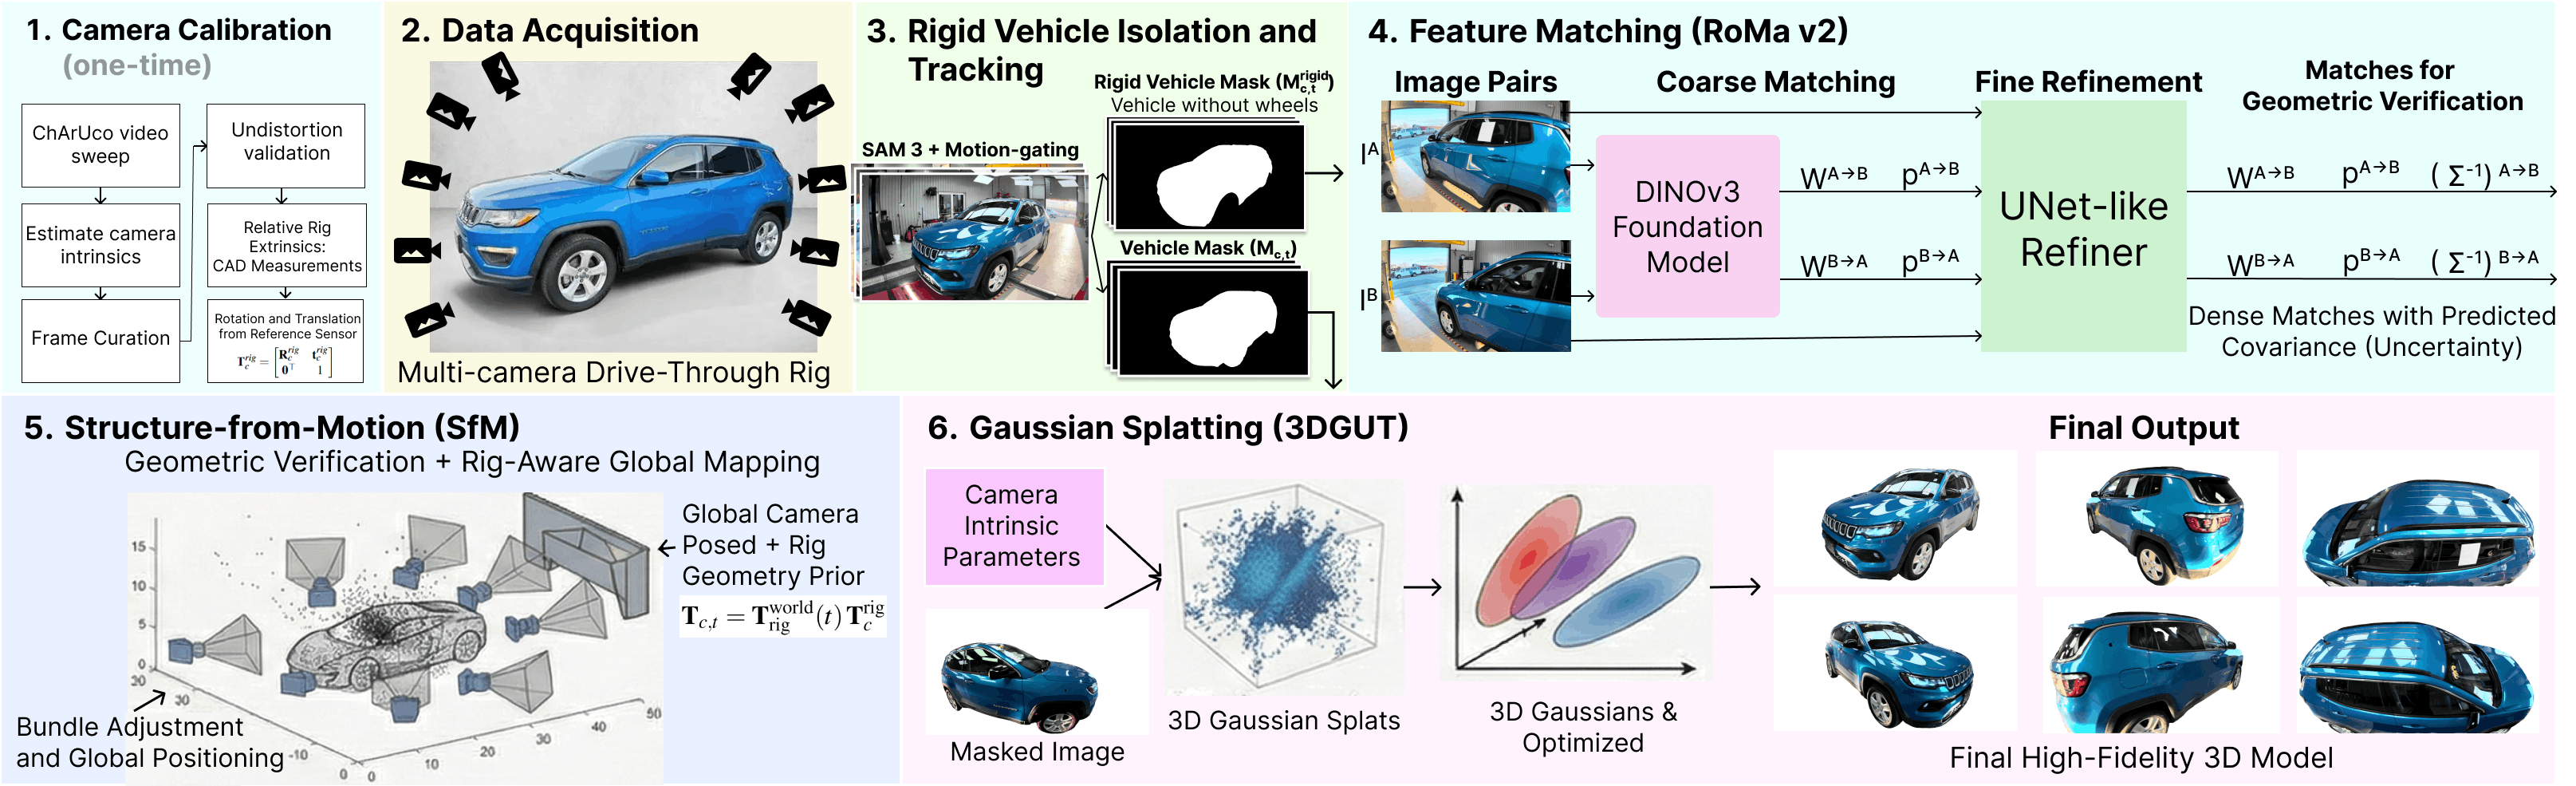
\includegraphics[width=\textwidth]{images_low/main_flowchart.png}
  \caption{\small \textbf{Overview of the proposed end-to-end 3D exterior reconstruction pipeline.} \textbf{(1) Camera Calibration:} One-time estimation of fisheye intrinsics and CAD-derived relative rig extrinsics. \textbf{(2) Data Acquisition:} Drive-through video capture of the moving vehicle using a 14-camera dual-pillar rig. \textbf{(3) Rigid Vehicle Isolation:} SAM 3 and motion-gating isolate the dynamic vehicle while explicitly subtracting non-rigid wheel rotations to satisfy epipolar constraints. \textbf{(4) Feature Matching:} The RoMa v2 learned matcher extracts robust dense correspondences directly on the raw, distorted frames. \textbf{(5) Structure-from-Motion (SfM):} Rig-aware global bundle adjustment geometrically verifies matches and estimates the camera poses using static structural hardware priors. \textbf{(6) Gaussian Splatting:} A distortion-aware 3D-GS architecture (3DGUT) renders the final photorealistic, interactive 3D model.}
  \label{fig:system_overview}
\end{figure*}

% Figure: 14-camera capture → masks → RoMAv2 matches → COLMAP Geometric verification + rig-aware global mapping → 3DGUT.

% label the mask uses:
% (A) Masking for RoMA v2 sampling + post-filtering (full image for context, then filter background matches)
% (B) Masking in Gaussian Splatting

% Successfully inverting the reference frame to reconstruct a moving vehicle within a static, cluttered dealership requires a tight integration of semantic disambiguation, robust learned correspondences, and physical hardware priors. To achieve this, we propose a modular, end-to-end pipeline tailored for multi-camera drive-through portals (Figure \ref{fig:system_overview}). 

Creating a high-quality 3D model from short drive-through videos of vehicles in cluttered dealerships requires inverting the frame of reference, integrating semantic disambiguation, robust learned correspondences, and hardware priors. We propose an end-to-end pipeline tailored for multi-camera drive-through rigs (Fig.~\ref{fig:system_overview}). Our pipeline converts videos into a high-quality 3D model of a vehicle. The process consists of six major steps. The first step (Sec.~\ref{subsec:methodology_camera_calibration}) is the one-time precise calibration of camera intrinsic and extrinsic parameters. The second step (Sec.~\ref{subsec:methodology_camera_rig_and_data_acquisition}) is the acquisition of drive-through videos of the vehicle. The third step isolates the dynamic vehicle from the dealership background via motion-gated semantic segmentation (Sec.~\ref{subsec:methodology_rigid_vehicle_isolation_and_tracking}). The fourth step generates feature correspondences directly on the raw, distorted frames (Sec.~\ref{subsec:methodology_feature_matching}). The fifth step (Sec.~\ref{subsec:methodology_structure_from_motion}) uses rig-aware SfM to geometrically verify these matches and estimate the sparse 3D geometry. The final step (Sec.~\ref{subsec:methodology_gaussian_splatting}) uses distortion-aware 3D Gaussian splatting to generate a photorealistic, interactive 3D model of the vehicle.


% The first step (Sec.~\ref{sub:camera_calibration}) is the precise calibration of camera intrinsic and extrinsic parameters to model wide-angle lens distortion and constrain global pose estimation. This calibration needs to be performed once; the calibrated camera parameters can be used to reconstruct 3D models of any vehicle.

% Let $\mathcal{I} = \{\mathbf{I}_{c,t}\}$ represent the raw 4K video from our two-pillar rig, where $c \in \{1, \dots, n\}$ indexes the \textit{n} cameras and $t$ indexes time. Each camera has calibrated fisheye intrinsics and a CAD-derived relative pose prior $\mathbf{T}^{\text{rig}}_{c} \in \mathrm{SE}(3)$. Our objective is to map $\mathcal{I}$ directly into a photorealistic 3D Gaussian Splatting representation without relying on destructive image undistortion.

% \begin{figure}[h]
%     \centering
%     \framebox[0.95\columnwidth]{
%         \begin{tabular}{c}
%              14-Camera 4K Capture Rig $\rightarrow$ Motion-Aware Semantic Masking \\
%              $\downarrow$ \\
%              RoMA v2 Learned Matching (Guided by Mask Set A) \\
%              $\downarrow$ \\
%              COLMAP Geometric Verification + Rig-Aware Global Mapping \\
%              $\downarrow$ \\
%              3DGUT Distortion-Aware Gaussian Splatting (Guided by Mask Set B)
%         \end{tabular}
%     }
%     \caption{End-to-end pipeline for dynamic vehicle exterior reconstruction. Semantic masks operate in two distinct branches: (A) \textit{Rigid-Body Masks} (excluding wheels) guide RoMA v2 sampling and post-filtering to satisfy SfM rigidity constraints; (B) \textit{Complete Vehicle Masks} (including wheels) supervise the Gaussian Splatting phase for visual fidelity.}
%     \label{fig:system_overview}
% \end{figure}

% \subsubsection{Motion-Aware Semantic Isolation}
% To resolve the dynamic-scene ambiguity, we compute a per-frame vehicle mask $M_{c,t} \in \{0,1\}^{H \times W}$ using SAM 3 instance proposals coupled with motion-gating and temporal consistency. Motion gating ensures that the selected instance corresponds to the vehicle passing between the camera pillars (and not a static background vehicle), while the temporal consistency prevents drift across frames. Because the vehicle's forward translation is physically coupled with the rotation of its wheels, applying a single mask universally induces geometric contradictions. For SfM, we explicitly subtract the wheel masks $W_{c,t}$ to form a rigid-body mask:
% \begin{equation}
% M^{\text{rigid}}_{c,t} \;=\; M_{c,t}\ \wedge\ \neg W_{c,t}
% \label{eq:rigid_mask}
% \end{equation}

% \subsubsection{Learned Matching on Distorted Imagery}
% We bypass exhaustive matching via a sparse spatial-temporal pair graph. RoMA v2 processes the raw image pairs, utilizing $M^{\text{rigid}}_{c,t}$ as a spatial confidence prior during sampling to bias candidate correspondences toward the rigid vehicle. Matches are assigned a confidence score $s = o \cdot p$ (overlap $o$, precision $p$) and aggressively post-filtered using grid-based thinning and mutual uniqueness to suppress specular degeneracies. 

% \subsubsection{Geometric Verification and Rig-Aware SfM}
% The filtered correspondences undergo two-view geometric verification. To combat scale drift across the wide cross-pillar baseline, we parameterize the global bundle adjustment by coupling camera poses through a shared rig trajectory:
% \begin{equation}
% \mathbf{T}_{c,t} \;=\; \mathbf{T}^{\text{world}}_{\text{rig}}(t)\,\mathbf{T}^{\text{rig}}_{c}
% \label{eq:rig_factorization}
% \end{equation}
% where $\mathbf{T}^{\text{world}}_{\text{rig}}(t)$ is the rig pose at time $t$. We run rig-aware global mapping and bundle adjustment to generate a consistent sparse point cloud and camera poses.

% \subsubsection{Distortion-Aware Gaussian Splatting}
% Finally, the optimized sparse geometry initializes 3DGUT, a distortion-aware Gaussian Splatting framework. We supervise the rendering optimization using the complete vehicle masks $M_{c,t}$ (which include the wheels) to prevent background artifacts:
% \begin{equation}
% \min_{\Theta}\ \sum_{c,t}\ \sum_{\mathbf{u}}
% M_{c,t}(\mathbf{u})\,
% \left\|\mathbf{I}_{c,t}(\mathbf{u}) - \hat{\mathbf{I}}_{c,t}(\mathbf{u};\Theta)\right\|_1
% \label{eq:masked_gs_loss}
% \end{equation}
% where $\hat{\mathbf{I}}_{c,t}(\cdot;\Theta)$ denotes the rendered image under Gaussian parameters $\Theta$.













\subsection{Camera Calibration and Camera Rig Pose Priors} 
\label{subsec:methodology_camera_calibration}
% # ChARUco Boards 

% ChArUco intrinsics (per-camera).

% Extrinsics prior from CAD (define rig frame, camera frames, parameterization).

% Explain what is held fixed vs refined in BA (I refine rig-from-world and sensor-from-rig). 

Integrating a multi-camera wide-baseline array into an SfM pipeline requires accurate geometric calibration, as small errors in wide-angle modeling propagate into noticeable structural drift. 

We first perform an offline calibration using large-format ChArUco boards to estimate the 8-parameter fisheye intrinsics, denoted $\boldsymbol{\theta}_c$, for each camera $c$. For normalized coordinates $(x,y)$ and radial distance $r = \sqrt{x^2+y^2}$, the distorted pixel coordinates $\mathbf{u}$ are computed as:
% \vspace{-2em}
\begin{equation}
    \theta = \arctan(r),\quad \theta_d = \theta(1 + k_1\theta^2 + k_2\theta^4 + k_3\theta^6 + k_4\theta^8)
\end{equation}
\begin{equation}
    \mathbf{u} = \begin{bmatrix} f_x (\theta_d / r) x + c_x \\ f_y (\theta_d / r) y + c_y \end{bmatrix}
\end{equation}
Because these parameters represent fixed physical properties of the lens-sensor assemblies, they are held strictly constant during all downstream geometric verification and bundle adjustment stages.

% Establishing the extrinsic spatial relationships across a wide drive-through portal solely via visual features is an underconstrained problem. To enforce structural rigidity, we define the left pillar's middle side camera as the origin of a generalized rig frame. We constrain the inter-camera extrinsics by injecting CAD-derived \emph{camera-from-rig} pose priors as static relative transforms in the rig frame:

% % , denoted $\bar{\mathbf{T}}^{\text{rig}}_{c} \in \mathrm{SE}(3)$. 
% \begin{equation}
%     \mathbf{T}_{c}^{rig} = \begin{bmatrix} \mathbf{R}_{c}^{rig} & \mathbf{t}_{c}^{rig} \\ \mathbf{0}^\top & 1 \end{bmatrix} \in SE(3)
% \end{equation}
% where $\mathbf{T}_{ref}^{rig}$ is the identity matrix.


% However, real-world deployment in active dealerships introduces minor mechanical variations due to installation tolerances and structural vibrations. Therefore, during global rig-aware bundle adjustment, we estimate the dynamic rig trajectory $\mathbf{T}^{\text{world}}_{\text{rig}}(t)$ while allowing a regularized, bounded refinement of the local static extrinsics: $
%     \mathbf{T}^{\text{rig}}_{c} = \exp(\boldsymbol{\xi}_c)\,\bar{\mathbf{T}}^{\text{rig}}_{c}, \qquad \boldsymbol{\xi}_c \in \mathfrak{se}(3).$
% This bounded relaxation effectively balances the global structural stability provided by the CAD priors with the photometric flexibility required to minimize the final reprojection error.









Estimating wide-baseline extrinsics solely from visual features is underconstrained \cite{guo2025robust}. We enforce structural rigidity by defining the left pillar's middle camera as the reference origin and injecting CAD-derived \emph{camera-from-rig} pose priors, denoted $\bar{\mathbf{T}}^{\text{rig}}_{c} \in \mathrm{SE}(3)$. 

Due to minor mechanical variations in real-world deployments (e.g., installation tolerances and structural vibrations), our global rig-aware bundle adjustment estimates the dynamic rig trajectory $\mathbf{T}^{\text{world}}_{\text{rig}}(t)$ while permitting a regularized, bounded refinement of these local extrinsics:$
    \mathbf{T}^{\text{rig}}_{c} = \exp(\boldsymbol{\xi}_c)\,\bar{\mathbf{T}}^{\text{rig}}_{c}, \qquad \boldsymbol{\xi}_c \in \mathfrak{se}(3).
$
This bounded relaxation optimally balances the global structural stability of the CAD priors with the photometric flexibility required to minimize reprojection error.












\subsection{Camera Rig and Data Acquisition}
\label{subsec:methodology_camera_rig_and_data_acquisition}
% Two-pillar geometry, 14 cameras, 4K@10FPS.

% Mention dealership environment and clutter explicitly (this motivates masking).

% We should include a tiny diagram defining:
% Rig frame origin (which camera is reference: Left Middle Side)
% Then connect it to COLMAP’s rig model: rigs assume fixed relative poses with one reference sensor.


% UPDATE THIS SECTION TO BE A BIT MORE GENERALIZABLE - FINAL DRAFT


% We use a custom-built, two-pillar drive-through rig to capture the full exterior of moving vehicles in a high-throughput commercial setting. The architecture consists of a left (driver's side) and right (passenger's side) pillar, each equipped with seven cameras capturing 4K video at 10 frames per second. The sensors span three elevations (bottom, middle, top) and three yaw orientations (front, side, rear) to maximize coverage in a single pass. 
% We extract all frames without temporal subsampling to preserve continuity for tracking and geometric estimation.


We collect the data using a two-pillar multi-camera drive-through rig to capture the full exterior of moving vehicles. Due to the short stand-off distance between the pillars and the vehicle, we use wide-FOV lenses. 
% We compute the camera intrinsic parameters using the fisheye model. For normalized coordinates $(x,y)$ and radial distance $r = \sqrt{x^2+y^2}$, the distorted pixel coordinates $\mathbf{u}$ are computed as:
% \begin{equation}
%     \theta = \arctan(r),\quad \theta_d = \theta(1 + k_1\theta^2 + k_2\theta^4 + k_3\theta^6 + k_4\theta^8)
% \end{equation}
% \begin{equation}
%     \mathbf{u} = \begin{bmatrix} f_x (\theta_d / r) x + c_x \\ f_y (\theta_d / r) y + c_y \end{bmatrix}
% \end{equation}
Instead of undistorting the frames, which severely degrades peripheral resolution, we retain the raw images and inject these exact intrinsic parameters directly into the downstream feature matching, bundle adjustment, and Gaussian splatting processes.

% To prevent structural drift across the wide cross-pillar baseline, we establish a fixed relative coordinate system. Designating the left pillar's middle side camera as the reference origin ($\mathbf{T}^{\text{rig}}_{\text{ref}} = \mathbf{I}$), each camera $c$ is constrained by an exact, CAD-derived static pose $\mathbf{T}^{\text{rig}}_{c} \in \mathrm{SE}(3)$. These physical priors formally link independent cameras into a cohesive generalized sensor.






































\subsection{Rigid Vehicle Isolation and Tracking}
\label{subsec:methodology_rigid_vehicle_isolation_and_tracking}

% Which name is better: 1. Dynamic Scene Disambiguation 2. Motion-Aware Semantic Segmentation 3. Rigid Vehicle Isolation and Tracking

% 3.4.1 Instance proposals from SAM3

% 3.4.2 Motion-gated target instance selection (anchor locked to the vehicle moving between the camera pillars)

% 3.4.3 Rigid-body mask construction for SfM (We also remove the wheels from the vehicle mask to further enhance structure-from-motion performance and remove dynamic objects.)

% 3.4.4 Rendering masks for Gaussian Splatting

% I use RoMA v2 with masks applied as confidence masks during sampling and also to filter out the final matches. First, passing in the entire image to give it the full context, including the background, and allow it to generate robust matches for symmetric objects (vehicle), and then I filter the matches from the background based on the masks.

% I am doing something crucial: subtracting the wheels from the vehicle mask. SfM fundamentally assumes a rigid scene. The car body is rigid; the rotating wheels are not. Explicitly state that removing the wheels is a mathematical necessity for accurate SfM, not just a cleanup step.

% % SfM assumes a static scene; using raw dealership images often causes the algorithm to lock onto the stationary, high-gradient background. To mathematically invert the reference frame, treating the moving vehicle as the static origin, we introduce a dynamic-scene disambiguation pipeline.

SfM algorithms assume a static environment and invariably lock onto the high-gradient dealership background rather than the moving vehicle. To overcome this and invert the reference frame, we introduce a dynamic-scene disambiguation pipeline that treats the vehicle as the static origin.


% \paragraph{Motion-Gated Instance Selection}

% % USE CHATGPT VERSION
% We generate zero-shot semantic instance proposals using the Segment Anything Model 3 (SAM 3) on the full, uncropped 4K frames. Because wholesale environments contain dense automotive clutter, a purely semantic approach is insufficient. We resolve this via a motion-gated tracking algorithm. By analyzing background-subtracted motion energy and temporal Intersection-over-Union (IoU) across sequential frames, the system anchors onto the specific vehicle traversing the portal and tracks it bidirectionally. Crucially, the system emits \textit{blank masks} for frames where the target vehicle has not yet entered or has already exited the specific camera's field of view, preventing the tracker from snapping to parked background cars.


\subsubsection{Motion-gated target selection and anchor-locked tracking}
For each frame $\mathbf{I}_{c,t}$, we query SAM~3 \cite{carion2025sam} with a text prompt (``car'') to obtain a set of instance proposals $\{S_{c,t}^{(i)}\}_{i=1}^{N_{c,t}}$, where each $S_{c,t}^{(i)}\in\{0,1\}^{H\times W}$ is a binary mask.

To bias selection toward the vehicle that traverses the capture volume, we compute a per-frame motion support mask $B_{c,t}\in\{0,1\}^{H\times W}$ using background subtraction (MOG2) \cite{zivkovic2004improved} followed by thresholding and morphological cleanup. We define a scalar motion energy
\begin{equation}
E_{c,t} \;=\; \frac{1}{|\Omega|}\sum_{\mathbf{u}\in\Omega} B_{c,t}(\mathbf{u}),
\label{eq:motion_energy}
\end{equation}
where $\Omega$ is the full image domain. We smooth $\{E_{c,t}\}$ with a moving average and choose an \emph{anchor frame} near peak motion while ignoring a fraction of frames at the sequence boundaries to accommodate front/rear cameras. Among the top-$K$ candidate anchor frames, we select the best instance by combining motion overlap, temporal consistency, and a weak size prior. Using the intersection-over-union
\begin{equation}
\mathrm{IoU}(A,B) \;=\; \frac{|A\cap B|}{|A\cup B|+\epsilon},
\label{eq:iou}
\end{equation}
the anchor/track selection score for instance $S_{c,t}^{(i)}$ is

% \begin{equation}
% \mathrm{score}\!\left(S_{c,t}^{(i)}\right) =
% 6\,\mathrm{IoU}\!\left(S_{c,t}^{(i)}, B_{c,t}\right)
% +2\,\mathrm{IoU}\!\left(S_{c,t}^{(i)}, M_{c,t-1}\right)
% +0.10\,\log(|S|+1)
% +0.75\,\mathrm{AreaSim}
% +0.25\,\mathrm{DetScore},
% \label{eq:sam_score}
% \end{equation}

\vspace{-1em}

\begin{equation}
\begin{split}
&\mathrm{score}\!\left(S_{c,t}^{(i)}\right) =
\,6\,\mathrm{IoU}\!\left(S_{c,t}^{(i)}, B_{c,t}\right)
+2\,\mathrm{IoU}\!\left(S_{c,t}^{(i)}, M_{c,t-1}\right) \\
&+0.10\,\log(|S|+1)
+0.75\,\mathrm{AreaSim}
+0.25\,\mathrm{DetScore},
\end{split}
\label{eq:sam_score}
\end{equation}
where $M_{c,t-1}$ is the previously selected mask, $|S_{c,t}^{(i)}|$ denotes the mask area in pixels, $\mathrm{AreaSim}$ measures similarity between the candidate area and a running reference area (to prevent drift to distant background vehicles), and $\mathrm{DetScore}$ is the model-provided instance confidence.

% We enforce $\mathrm{IoU}(S_{c,t}^{(i)}, M_{c,t-1}) \ge \tau_{\text{track}}$ and stop tracking after $G$ consecutive failures.

Starting from the anchor, we track backward and forward in time with a \emph{strict lock} enforcing $\mathrm{IoU}(S_{c,t}^{(i)}, M_{c,t-1}) \ge \tau_{\text{track}}$ and an anti-drift size constraint (minimum area ratio relative to a running reference). If tracking fails for more than $G$ consecutive frames, we stop in that direction and later write \emph{blank masks} for all frames outside the final active interval. Short false gaps in the 1D presence signal are filled via temporal closing to handle brief occlusions or near-stops. This anchor-locked design is required in dealership lanes, where static background cars can otherwise become the dominant instance when the target vehicle is absent.


\subsubsection{Rigid-Body Mask Construction}
SfM assumes a rigid scene; however, the vehicle's forward translation is coupled with the rotation of its wheels. If wheel keypoints are incorporated into the bundle adjustment, their independent trajectories violate the epipolar constraint ($\mathbf{x}_i^\top \mathbf{E} \mathbf{x}_j = 0$), inducing structural drift. Therefore, we explicitly segment and subtract the wheel masks $W_{c,t}$ from the tracked vehicle mask $M_{c,t}$ to enforce rigidity:
\begin{equation}
    M^{\text{rigid}}_{c,t} = M_{c,t} \wedge \neg W_{c,t}
\end{equation}
% This subtraction is a strict mathematical necessity for stable SfM convergence, not merely a heuristic cleanup.

\subsubsection{Bifurcated Mask Utilization}
This rigid-body mask $M^{\text{rigid}}_{c,t}$ serves as a probabilistic spatial confidence prior during the subsequent RoMA v2 \cite{edstedt2025roma} matching phase, guiding the network to sample features exclusively on the rigid car body. However, because the final 3D model presented to customers must be visually complete, we define a secondary rendering mask $M^{\text{render}}_{c,t} = M_{c,t}$ that explicitly retains the wheels. This full mask is passed forward to define the visual foreground during the final Gaussian Splatting optimization.


% \begin{figure}
%     \centering    \includegraphics[width=1\linewidth]{images/rigid_vehicle_isolation_and_tracking.png}
%     \caption{Rigid Vechicle Isolation and Tracking}    \label{fig:rigid_vehicle_isolation_and_tracking}
% \end{figure}

% \begin{figure}[t]
%     \centering    \includegraphics[width=1\linewidth]{images/data_collection_1.png}
%     \caption{Data Collection}    \label{fig:data_collection}
% \end{figure}


\subsection{Feature Matching}

\label{subsec:methodology_feature_matching}

% Which image pairs are matched?

% Intra-frame across cameras?

% Temporal neighbors within camera?

% Cross-camera temporal offsets allowed?

% How do you avoid combinatorial explosion?

% You don’t need a huge section, just a clear one:

% define pair graph construction

% explain overlap prior / rig-based adjacency / temporal window

% explain why exhaustive matching is not used

\subsubsection{Image Pair Graph Generation}

% A drive-through inspection yields a total image set $\mathcal{V}$ containing approximately 1,400 high-resolution 4K frames.

Matching features across a multi-camera capture system is computationally expensive. A naive SfM pipeline uses exhaustive matching, which scales quadratically as $\mathcal{O}(|\mathcal{V}|^2)$ and is geometrically redundant; attempting to match most opposing cross-pillar cameras yields few verified inliers due to the vehicle body occluding the line of sight as it passes directly in front of the cameras.

We construct a constrained pair graph $\mathcal{G} = (\mathcal{V}, \mathcal{E})$ to prevent this combinatorial explosion while ensuring robust geometric connectivity. The edges $\mathcal{E}$ define the exact image pairs passed to the learned matcher, formulated as the union of spatial and temporal connections:
$
    \mathcal{E} = \mathcal{E}_{\text{spatial}} \cup \mathcal{E}_{\text{temporal}}.
$

The spatial edges ($\mathcal{E}_{\text{spatial}}$) connect concurrent frames from different cameras based on visual overlap derived directly from the physical rig prior. We enforce a strict adjacency matrix $\mathbf{A} \in \{0,1\}^{C \times C}$ where $\mathbf{A}_{k,j} = 1$ only if camera $k$ and $j$ share a field of view. This includes adjacent sensors on the same pillar, and the cross-pillar overlap between the left and right top side cameras, which bridges the two pillars into a single connected component. We set $\mathbf{A}_{k,j} = 0$ for all other cross-pillar pairs to avoid computing fully occluded matches. We use a bounded temporal offset $\Delta \in [-K, K]$ around these cross-camera matches to improve robustness:
\begin{equation}
    \mathcal{E}_{\text{spatial}} = \left\{ (I_{k,t}, I_{j,t+\Delta}) \mid \mathbf{A}_{k,j} = 1, \Delta \in [-K, K] \right\}
\end{equation}

The temporal edges ($\mathcal{E}_{\text{temporal}}$) connect sequential frames within the same camera to track the vehicle's forward translation using a sliding window $\tau$:
\begin{equation}
    \mathcal{E}_{\text{temporal}} = \left\{ (I_{k,t_1}, I_{k,t_2}) \mid |t_1 - t_2| \leq \tau \right\}
\end{equation}

This bounded-degree construction reduces the number of matched pairs from $\mathcal{O}(|\mathcal{V}|^2)$ to
$|\mathcal{E}|=\mathcal{O}\!\big(|\mathcal{V}|\tau + |\mathcal{V}|\,d(2K+1)\big)$,
i.e., linear in $|\mathcal{V}|$ for fixed windows, while maintaining sufficient connectivity for robust rig-aware SfM.









\subsubsection{Learned Feature Matching}
% \label{sec:learned_matching}

% 3.4.1 (Correspondence generation with RoMA v2)

% Be explicit that I export correspondences into COLMAP rather than relying on COLMAP’s matcher. My script: confidence masks during sampling, mask filtering, grid thinning, mutual uniqueness, then writes matches.txt for COLMAP matches_importer to do Geometric Verification.


% 3.4.2 Geometric verification in COLMAP (two-view geometry + rig verification)

% Your parameters are concrete; list the important ones (max_error, min_inliers, inlier_ratio, rig_verification).

% Filters: score threshold, grid thinning, quantization, mutual uniqueness (one-to-many suppression) 
% Writes matches.txt in COLMAP’s expected format and inserts keypoints (dummy descriptors) into the DB
% That’s worth a short algorithm box (“Match Export + Post-filtering”) because it’s one of your core contributions.

% I am applying the vehicle masks as confidence masks to the RoMA overlap tensors before sampling. This is a brilliant technical detail because it gives the matcher full image context while forcing it to sample points only on the vehicle. This deserves a dedicated paragraph or an Algorithm Box.

% The Post-Filtering Pipeline: Detail the grid-based thinning and mutual uniqueness constraints. Reviewers love seeing how learned models are tamed for classical geometric verification.


% I am not just “using RoMa v2.”
% I am doing a structured match pipeline:

% confidence-mask-aware sampling

% score filtering

% mutual uniqueness (one-to-one suppression)

% grid thinning

% export to COLMAP DB + matches.txt

% then geometric verification in COLMAP

% That deserves an algorithm box or pseudo-code block like:

% Algorithm 1: Motion- and Mask-Aware RoMa v2 Match Export for COLMAP


The combination of fisheye lens distortion and the highly reflective, specular nature of automotive paint renders classical feature extractors inadequate. We use RoMA v2, a dense learned matcher that generates robust matches across these challenging surfaces.

% A critical innovation in our pipeline is the method by which we integrate the rigid vehicle masks, $M^{\text{rigid}}$, into the deep matching process. 
If the frames were cropped or masked prior to network inference, the transformer layers would lose the global visual context required to resolve ambiguities across symmetric automotive panels. Instead, we pass the full, un-undistorted image pairs $(I_A, I_B)$ through the network. We then apply our semantic masks as confidence priors directly to the network's internal overlap tensors before the dense sampling phase:
\begin{equation}
    \tilde{O}_A(\mathbf{u}) = O_A(\mathbf{u}) \cdot M^{\text{rigid}}_A(\mathbf{u})
\end{equation}
This forces the network to sample keypoints on the rigid vehicle body while utilizing the full spatial receptive field.

Once the raw correspondences are sampled, we enforce strict epipolar constraints. Matches are assigned a confidence score $s_i = o_i \cdot \min(p^{A\rightarrow B}_i, p^{B\rightarrow A}_i)$ and subjected to a hard score threshold. To combat the one-to-many match errors frequently caused by identical specular highlights, we enforce mutual uniqueness, suppressing all non-bijective mappings. We apply grid-based spatial thinning, retaining the highest-scoring match per spatial cell to ensure a uniform distribution of structural constraints and prevent the bundle adjustment from being biased toward highly textured regions. We then perform two-view geometric verification using RANSAC~\cite{fischler1981random} to generate the verified inliers (Alg. \ref{alg:roma_export}).






\begin{algorithm}[t]
\caption{Motion- and Mask-Aware RoMA v2 Matching}
\label{alg:roma_export}
\begin{algorithmic}[1]
\REQUIRE Pair graph $\mathcal{E}$, images $\{I_k\}$, rigid masks $\{M^{\text{rigid}}_k\}$, thresholds $(\tau_s, g, K, q, N_{\max})$
\FOR{each pair $(A, B) \in \mathcal{E}$}
    \STATE Run RoMA v2 forward pass on $(I_A, I_B)$ to obtain prediction structure with overlap and precision maps $\{O_A, O_B, P^{A\rightarrow B}, P^{B\rightarrow A}\}$
    % \STATE Resize rigid masks to the map resolution: $\hat{M}^{\text{rigid}}_A,\hat{M}^{\text{rigid}}_B$
    \STATE Apply confidence-mask sampling weights: $\tilde{O}_A \leftarrow O_A \odot M^{\text{rigid}}_A$
    \STATE Sample raw correspondences based on $\tilde{O}_A$; compute symmetric confidence scores $s_i = o_i \cdot \min(p^{A\rightarrow B}_i, p^{B\rightarrow A}_i)$
    % \STATE Retain matches where $s_i \geq \tau_s$; retain only points inside $M^{\text{rigid}}_A$ and $M^{\text{rigid}}_B$
    \STATE Retain matches with $s_i \geq \tau_s$ that fall inside $M^{\text{rigid}}_A$ and $M^{\text{rigid}}_B$
    \STATE Keep top-$K$ matches per $g \times g$ spatial cell
    \STATE Quantize coordinates by $q$ and suppress one-to-many and many-to-one matches; cap total to $N_{\max}$
\ENDFOR
\STATE Perform geometric verification on the filtered matches
\end{algorithmic}
\end{algorithm}









\subsection{Structure-from-Motion (SfM)}

\label{subsec:methodology_structure_from_motion}

%  3.4.3 Rig-aware mapping / bundle adjustment

% My undercarriage paper explained the rig-aware regularization conceptually; for the new paper, connect that to the 14-cam CAD priors + COLMAP rig tools. I also use the GLOBAL mapper here.



% Translating isolated two-view geometries into a globally consistent 3D structure across a dual-pillar setup presents a significant challenge. 
Incremental SfM sequentially registers images, which can result in scale drift across the wide physical baseline when relying solely on visual features from a specular, moving vehicle. We use a Global SfM strategy \cite{pan2024global} with integrated hardware priors to construct an accurate point cloud.

The absolute pose of any camera $c$ at time $t$ is factorized into a dynamic global trajectory and a static local offset:
\begin{equation}
    \mathbf{T}_{c,t} = \mathbf{T}^{\text{world}}_{\text{rig}}(t)\,\mathbf{T}^{\text{rig}}_{c}
    \label{eq:rig_factor}
\end{equation}
Here, $\mathbf{T}^{\text{world}}_{\text{rig}}(t) \in \mathrm{SE}(3)$ describes the motion of the generalized multi-camera rig relative to the stationary vehicle, and $\mathbf{T}^{\text{rig}}_{c} \in \mathrm{SE}(3)$ represents the static offset of camera $c$ from the reference sensor.



By using a global mapper, we simultaneously optimize the 3D structure $\mathbf{X}$ and the network of camera poses, closing the loop between the two pillars instantly. The optimization minimizes the global reprojection error:
\begin{equation}
\begin{aligned}
\arg\min_{\mathbf{X}, \mathbf{T}^{\text{world}}_{\text{rig}}, \mathbf{T}^{\text{rig}}_{c}}
&\sum_{(c,t),j} \rho \!\left(
\left\| \pi_c \!\left( \mathbf{T}^{\text{world}}_{\text{rig}}(t)\, \mathbf{T}^{\text{rig}}_{c}\, \mathbf{X}_j \right)
- \mathbf{x}_{c,t,j} \right\|_2^2
\right) \\
&\quad + \lambda \sum_{c} d \!\left( \mathbf{T}^{\text{rig}}_{c}, \bar{\mathbf{T}}^{\text{rig}}_{c} \right)
\end{aligned}
\end{equation}

where $\rho(\cdot)$ is the Huber loss function, utilized to mitigate the influence of false-positive correspondence outliers without destabilizing the convergence. Here, $\pi_c$ denotes the non-linear fisheye projection, $\mathbf{x}_{c,t,j}$ is the 2D pixel coordinate, and $d(\cdot, \cdot)$ is a quadratic pose deviation penalty enforcing the physical hardware constraints.


While the initial local offsets $\bar{\mathbf{T}}^{\text{rig}}_{c}$ are seeded directly from CAD measurements, they are not held absolutely rigid. The $\lambda$ penalty permits a tightly bounded parameter relaxation, allowing the bundle adjuster to refine local extrinsics alongside the global vehicle trajectory to account for microscopic real-world installation tolerances. This yields a dense, accurate, sparse point cloud.










\subsection{Gaussian Splatting}
\label{subsec:methodology_gaussian_splatting}


% I use 3DGUT, which supports fisheye camera models.

% We use vehicle masks (with wheels included for Gaussian Splatting) with 3DGUT. We pass the masks to the 3DGUT pipeline.

% We also use MCMC strategy.

% Explain why 3DGUT (with its fisheye/distortion support) and MCMC strategies allow you to retain the raw 4K quality all the way to the end.

% The rig-aware SfM stage yields a metrically consistent sparse point cloud aligned to the moving vehicle. 
We transition to a dense volumetric representation to synthesize photorealistic, interactive novel views of the vehicle exterior. Standard 3D Gaussian Splatting (3D-GS) architectures assume an ideal pinhole camera model. Forcing our dual-pillar dataset into standard 3D-GS requires pre-undistorting the 4K frames, which degrades the high-frequency visual information required to faithfully reproduce the micro-textures that are crucial for dealership inspections.

To retain the uncompressed 4K quality, we use 3DGUT \cite{wu20253dgut}, a distortion-aware Gaussian Splatting framework. In standard 3D-GS, the projection of a 3D Gaussian covariance $\bm{\Sigma} \in \mathbb{R}^{3 \times 3}$ to the 2D image plane relies on the Jacobian of the affine pinhole projection. 3DGUT replaces this approximation with an Unscented Transform (UT) that supports the highly non-linear fisheye projection optimized during SfM. For a 3D Gaussian $(\boldsymbol{\mu},\boldsymbol{\Sigma})$, UT forms sigma points:
\begin{equation}
    \mathbf{X}_0=\boldsymbol{\mu}, \qquad \mathbf{X}_{k}=\boldsymbol{\mu}\pm \left(\sqrt{(d+\lambda)\boldsymbol{\Sigma}}\right)_k,\ \ k=1,\dots,d
\end{equation}
These points are projected using the true fisheye camera model, $\mathbf{u}_k=\pi(\mathbf{K},\mathbf{T},\mathbf{X}_k)$, allowing the projected 2D covariance $\mathbf{S}$ to be approximated:
\begin{equation}
    \mathbf{S}=\sum_{k} w_k(\mathbf{u}_k-\hat{\mathbf{u}})(\mathbf{u}_k-\hat{\mathbf{u}})^{\top}
\end{equation}
This allows 3DGUT to rasterize directly onto the raw, distorted image plane.



Because automotive clear coats are reflective, standard splat densification heuristics often become trapped in local minima, resulting in floating artifacts. We use the Markov Chain Monte Carlo (MCMC) strategy, which reframes densification as a stochastic sampling problem to explore the parameter space. We supervise the 3DGUT optimization using the complete vehicle masks $M^{\text{render}}_{c,t}$ (which include the wheels) to ensure visual completeness of the final 3D model.
















\section{Experiments} 
We validate our end-to-end 3D reconstruction pipeline using a dataset captured from 10 automotive dealerships in five states across the USA. All experiments were executed on a workstation equipped with an AMD EPYC 7763 CPU, 2 TB of RAM, and eight NVIDIA RTX A6000 GPUs. 

\subsection{Camera Calibration } 
\label{subsec:experiments_camera_calibration}

Our experimental framework is built upon data captured from operational dealerships to maintain real-world relevance. We utilize a dual-pillar imaging system, with each pillar housing a seven-camera array. We calibrated 8-parameter fisheye camera models using a ChArUco board, achieving a sub-pixel mean root-mean-square (RMS) reprojection error of $0.42$ pixels at 4K resolution across all 14 cameras.
% This high fidelity justifies our decision to hold the intrinsic parameters strictly constant during downstream global mapping. 

 We tracked the deviation of the \textit{sensor-from-rig} transforms after the rig-aware bundle adjustment converged, to evaluate the stability of our CAD-derived extrinsic priors ($\bar{\mathbf{T}}^{\text{rig}}_{c}$). The optimization yielded a mean translational shift of $12.4$ mm and a mean rotational deviation of $0.8^\circ$ across the 13 non-reference cameras. 
 
 % These bounded, millimeter-scale deviations confirm a critical hypothesis: while the initial CAD measurements successfully prevented structural collapse across the wide $3.52$ m cross-pillar baseline, permitting bounded parameter relaxation was mathematically necessary to absorb real-world mechanical installation tolerances without forcing structural errors into the photometric reprojection.








\subsection{Data Acquisition and Deployment Conditions}
\label{subsec:experiments_data_acquisition_and_deployment_conditions}

% #vehicles, makes/models, lighting variability, dealership clutter types, capture duration.
% We use a custom-built, two-pillar drive-through rig to capture the full exterior of moving vehicles in a high-throughput commercial setting. The architecture consists of a left (driver's side) and right (passenger's side) pillar, each equipped with seven cameras capturing 4K video at 10 frames per second. The sensors span three elevations (bottom, middle, top) and three yaw orientations (front, side, rear) to maximize coverage in a single pass. 

We use a two-pillar 14-camera rig deployed in active dealership service lanes (Fig.~\ref{fig:data_collection}). The distance between the pillars is 140 inches. We collected a dataset of $N=25$ unique vehicles spanning diverse geometries (sedans, SUVs, trucks) and paint finishes. The capture duration averages 10 seconds per drive-through. Given our capture rate of 10 frames per second (FPS), each vehicle instance yields an uncompressed 4K spatio-temporal image tensor:
\begin{equation}
    \mathcal{I}^{(n)} = \left\{ \mathbf{I}^{(n)}_{c,t} \right\} \in \mathbb{R}^{14 \times T_n \times H \times W \times 3}
\end{equation}
where $c \in \{1, \dots, 14\}$ indexes the cameras, $T_n \approx 100$ represents the temporal frame count, and $(H, W) = (2160, 3840)$. This results in approximately $1400$ raw frames per capture. 



% \begin{figure}[t]
%     \centering    
\includegraphics[width=1\linewidth]{images/data_collection.png}
%     \caption{Data Collection}    \label{fig:data_collection}
% \end{figure}

\begin{figure}[t]
    \centering
    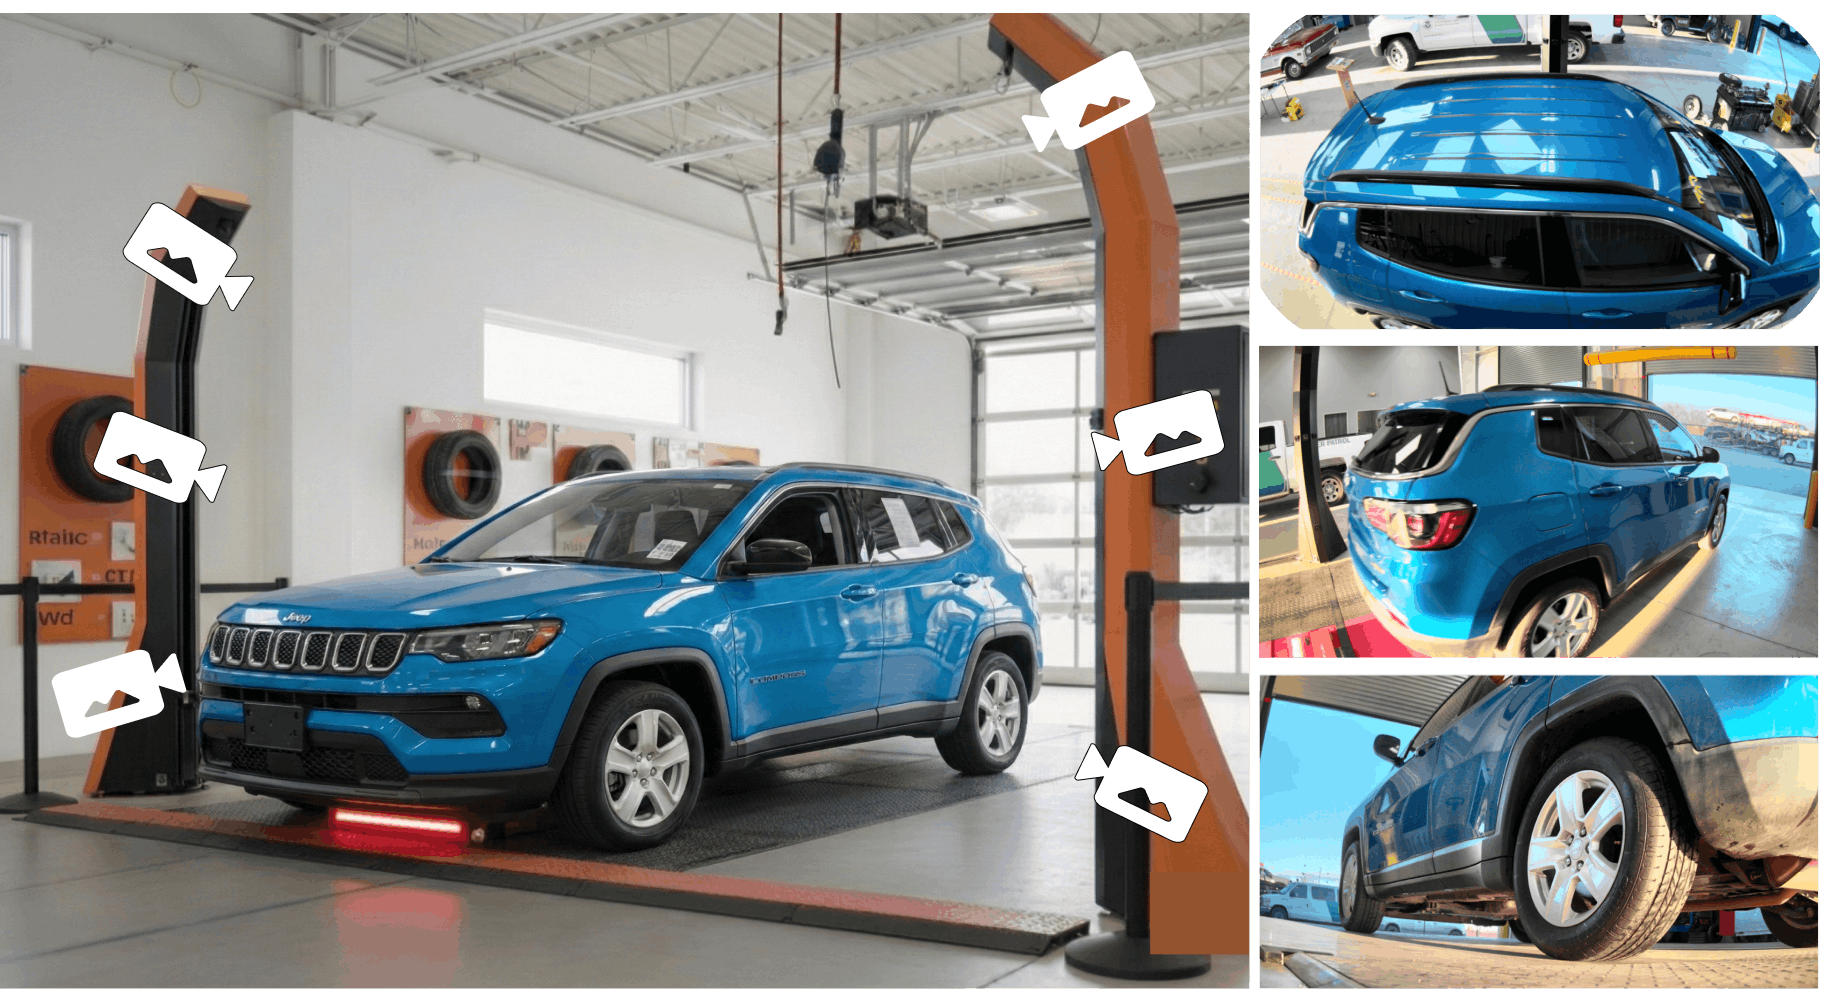
\includegraphics[width=1\linewidth]{images_low/data_collection.png}
    \caption{\small Data collection in a commercial dealership. The 14-camera dual-pillar rig captures 4K video as the vehicle traverses the highly cluttered, unconstrained capture volume. To maximize coverage in a single pass, cameras are mounted on both the driver's and passenger's sides across three vertical tiers (16, 55, and 97 inches), featuring front-, side-, and rear-facing yaw orientations.}
    \label{fig:data_collection}
\end{figure}






















% \subsection{Rigid Vehicle Isolation and Tracking}
% \begin{figure}
%     \centering    \includegraphics[width=1\linewidth]{images/rigid_vehicle_isolation_and_tracking.png}
%     \caption{Rigid Vechicle Isolation and Tracking}    \label{fig:rigid_vehicle_isolation_and_tracking}
% \end{figure}





% \subsection{Feature Matching}
% Figure~\ref{fig:roma_v2_matches} visualizes RoMA~v2 correspondences \cite{edstedt2025romav2} after applying our rigid-body masks. Two aspects are critical in this drive-through setting: (i) masking suppresses the high-gradient stationary background that otherwise dominates matching, and (ii) the resulting match graph retains global connectivity across the portal (including selected cross-pillar pairs with consistent overlap) to avoid disconnected reconstruction components. 













\subsection{Rigid Vehicle Isolation and Tracking}
\label{subsec:experiments_rigid_vehicle_isolation_and_tracking}

% To evaluate the efficacy of our dynamic-scene disambiguation, we qualitatively analyze the outputs of the motion-gated semantic masking module. 
Fig.~\ref{fig:rigid_vehicle_isolation_and_tracking} illustrates the temporal progression of the vehicle mask across a single camera view. Motion-gated SAM 3 segmentation identifies the primary moving target while entirely suppressing the dense, dealership background and parked distractor vehicles. Tracking successfully handles sequence boundaries; as the vehicle exits the camera's field of view, the system correctly emits blank masks rather than drifting onto background clutter. By excluding these non-rigid components, the resulting masks ensure that all downstream SfM constraints adhere to the rigid-body assumption.

% \begin{figure}[ht]
%     \centering
%     \includegraphics[width=1\linewidth]{images/rigid_vehicle_isolation_and_tracking.png}
%     \caption{Rigid Vehicle Isolation and Tracking. The motion-gated SAM 3 pipeline tracks the dynamic vehicle while suppressing background dealership clutter and explicitly masking out the non-rigid rotating wheels.}
%     \label{fig:rigid_vehicle_isolation_and_tracking}
% \end{figure}

\begin{figure}[ht]
    \centering
    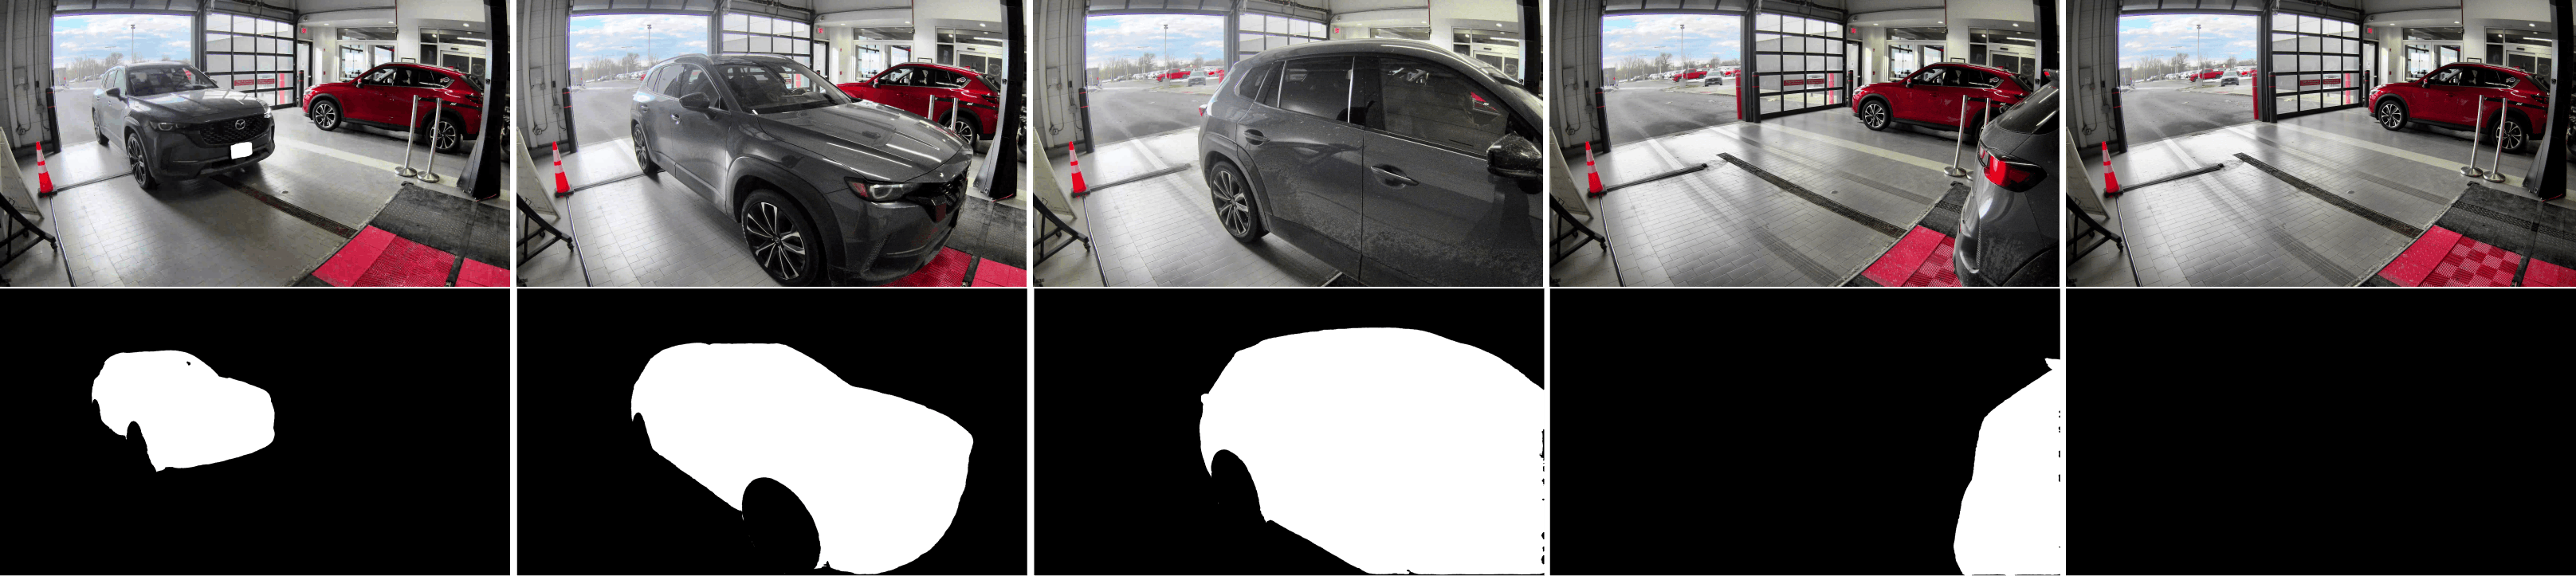
\includegraphics[width=1\linewidth]{images_low/rigid_vehicle_isolation_and_tracking_2.png}
    \caption{\small Rigid vehicle isolation and tracking. Top: representative frames. Bottom: corresponding rigid-body masks produced by motion-gated SAM 3 tracking. The pipeline tracks the dynamic vehicle while suppressing background dealership clutter and explicitly masking out the non-rigid rotating wheels.}
    \label{fig:rigid_vehicle_isolation_and_tracking}
\end{figure}












\subsection{Feature Matching}
\label{subsec:experiments_feature_matching}
% Generating valid correspondences in this environment is exceptionally difficult due to the highly specular, textureless nature of automotive clear coats, which easily confound classical feature extractors.

Fig.~\ref{fig:roma_v2_matches} visualizes RoMA~v2 correspondences after applying our rigid-body masks and post-filtering algorithms. Masking suppresses the high-gradient stationary background that otherwise dominates matching. The resulting match graph retains global connectivity across the portal (including selected top camera cross-pillar pairs with consistent overlap) to avoid disconnected reconstruction components. By injecting the rigid-body masks as confidence priors during RoMA v2's sampling phase, the network successfully concentrates keypoints exclusively on the dynamic vehicle. Because we do not hard-crop the images, the network retains the global visual context required to resolve ambiguities across symmetric automotive panels. 

\begin{figure}[t]
    \centering
    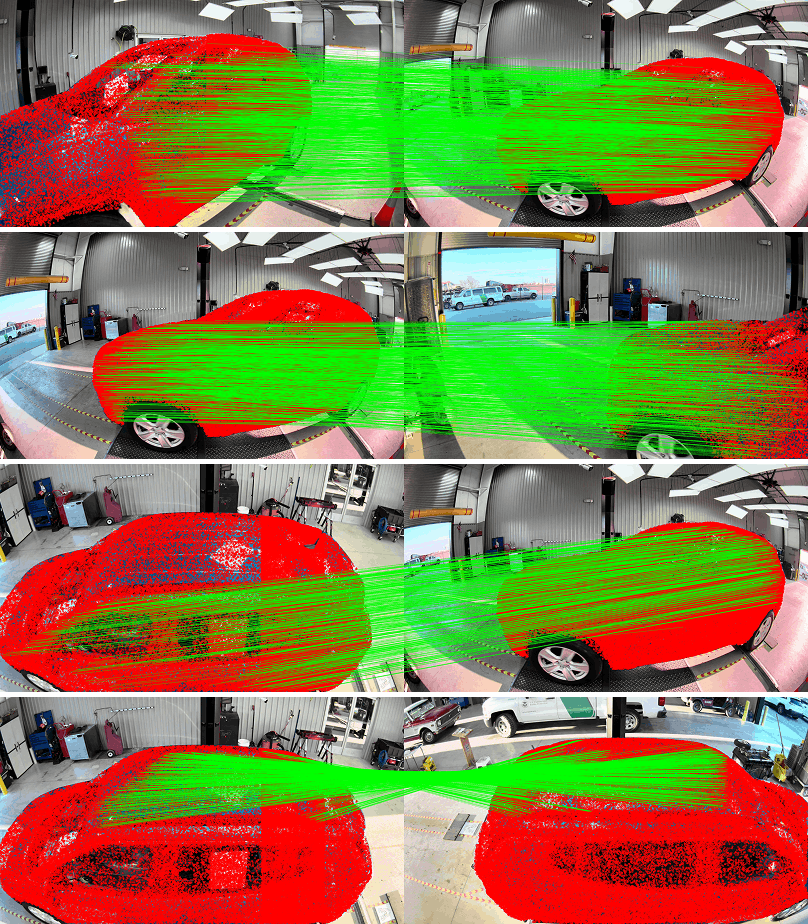
\includegraphics[width=\linewidth]{images_low/RoMA_v2.png}
    \caption{\small RoMA~v2 correspondence visualization on distorted images after rigid-body masking. The dense green correspondence lines confirm that the learned matcher successfully bridges extreme viewpoint changes on the raw 4K frames, overcoming wide-FOV fisheye distortion.}
    \label{fig:roma_v2_matches}
\end{figure}

% Furthermore, the dense green correspondence lines confirm that the learned matcher successfully bridges extreme viewpoint changes directly on the raw 4K frames, overcoming severe wide-FOV fisheye distortion without relying on destructive pre-undistortion.










% \subsection{Rigid Vehicle Isolation and Tracking}
% \label{sec:exp_masks}

% Because our capture occurs in active dealerships with a moving target and a static, high-gradient background, vehicle isolation is a prerequisite for reliable correspondence generation and subsequent SfM. We evaluate the masking stage qualitatively by inspecting per-camera mask sequences across representative passes, focusing on three failure modes that commonly break static-scene SfM: (i) \emph{instance drift} to other vehicles or background structures, (ii) \emph{temporal inconsistency} (flicker) that causes unstable constraints across frames, and (iii) \emph{incorrect presence} when the target vehicle is out of view (e.g., early frames for rear-facing cameras and late frames for front-facing cameras).

% Figure~\ref{fig:rigid_vehicle_isolation_and_tracking} shows example frames and the corresponding rigid-body masks produced by our motion-gated SAM~3 tracking module. The masks remain locked to the vehicle traversing the portal despite background clutter and varying viewpoint, and they correctly emit blank/partial masks near sequence boundaries where the vehicle is only partially observed. For SfM, we additionally remove wheels to satisfy rigidity assumptions; while this excludes rotating wheel texture from geometric estimation, it reduces non-rigid outliers that otherwise degrade two-view verification and bundle adjustment.

% We emphasize that the primary role of this module is not to achieve pixel-perfect segmentation, but to provide a \emph{high-precision foreground support} that suppresses background-dominated matches. The impact of this design choice is reflected downstream in Section~\ref{sec:exp_sfm}: ablations without motion-aware masks are substantially more likely to lock onto the static environment and fail to recover a vehicle-centric sparse model.

% \begin{figure}[t]
%     \centering
%     \includegraphics[width=\linewidth]{images/rigid_vehicle_isolation_and_tracking.png}
%     \caption{Rigid vehicle isolation and tracking. Top: representative frames from different cameras and times. Bottom: corresponding rigid-body masks produced by motion-gated SAM~3 tracking (wheels removed for SfM).}
%     \label{fig:rigid_vehicle_isolation_and_tracking}
% \end{figure}


% \subsection{Feature Matching}
% \label{sec:exp_matching}

% We evaluate learned correspondence quality qualitatively because the ground-truth dense correspondence field is unavailable for real dealership imagery. Instead, we assess whether the matcher produces (i) \emph{vehicle-centric} correspondences after masking, (ii) \emph{spatial coverage} over large rigid regions (doors, quarter panels, roofline), and (iii) \emph{graph connectivity} sufficient to link frames across time and across cameras in the portal.

% Figure~\ref{fig:roma_v2_matches} visualizes RoMA~v2 correspondences \cite{edstedt2025romav2} on distorted portal imagery after applying rigid-body masking. The key qualitative observation is that the correspondences concentrate on the vehicle silhouette and major rigid structures rather than on the background, which is critical in this dynamic-capture regime. In addition, we include cross-camera matches among overlapping viewpoints (including selected cross-pillar pairs with consistent overlap) to avoid disconnected components in the correspondence graph. This connectivity is necessary to propagate constraints across the two pillars and to support rig-aware global mapping.

% Finally, we note that automotive exteriors exhibit strong view-dependent reflectance; as a result, some regions (e.g., mirror-finish black panels) can yield sparse or unstable matches. In our pipeline, this is mitigated by (i) using RoMA~v2 on raw distorted images for robustness under wide-FOV optics and (ii) subsequent two-view geometric verification that filters remaining outliers before global optimization. The downstream effect of these correspondences is quantified in Section~\ref{sec:exp_sfm} through registration rate, sparse point density, and reprojection error.

% \begin{figure}[t]
%     \centering
%     
\includegraphics[width=\linewidth]{images/RoMA_v2.png}
%     \caption{RoMA~v2 correspondence visualization \cite{edstedt2025romav2} on distorted portal imagery after rigid-body masking. Dense, mask-guided matches provide vehicle-centric constraints and maintain graph connectivity for downstream two-view verification and global reconstruction.}
%     \label{fig:roma_v2_matches}
% \end{figure}




























% \subsection{Structure-from-Motion}
% \label{sec:exp_sfm}

% % Use (and update) what worked before: registered images, sparse points, reprojection error, Mean track length. 

% % Here, we'll add the ablation studies:

% % 4.3 Masking Ablations 

% % At least:

% % No masks

% % SAM3-only masks

% % SAM3 + motion-gated instance selection (our full method) 



% % Report: registration rate, reprojection error, and qualitative failure modes.

% % 4.4 Matching Ablations

% % DSP SIFT and COLMAP matcher baseline vs RoMA v2 (show why RoMA v2 matters on exterior + wide-FOV + reflections).

% % With/without your match post-filters (grid thinning + mutual uniqueness). 



% % 4.5 Rig Prior Ablations

% % With CAD prior vs without (or weak prior).

% % Also, show robustness: does it reduce inter-camera drift? (previous paper explicitly sold rig-aware BA as preventing drift).

% % One grid, 6–8 panels:
% % Success case
% % Failure due to low motion energy (mask suppression)
% % Failure due to heavy reflections
% % Failure due to poor coverage (occlusion)
% % This makes our masking and match filters feel necessary (not heuristic).
% Having established a robust mathematical foundation through intrinsic calibration and rigid extrinsic priors, we evaluate the system's ability to extract the dynamic vehicle geometry. The primary objective of the SfM phase is to generate a metrically accurate sparse point cloud to initialize the neural rendering. We evaluate the pipeline across four metrics: registration rate ($R_{reg}$), total validated sparse points ($N_{pts}$), mean track length ($L_{track}$), and mean reprojection error ($E_{reproj}$). 

% To overcome the photometric challenges of automotive clear coats and extreme fisheye distortion, our pipeline relies on RoMA v2. As demonstrated in Figure \ref{fig:roma_v2_matches}, applying semantic confidence masks during the sampling phase ensures that the network successfully establishes dense, robust correspondences directly on the moving vehicle body while strictly ignoring the dealership clutter.

% To isolate our architectural contributions, we conducted comprehensive ablations on masking, learned matching, and rig-aware optimization, summarized in Table \ref{tab:sfm_ablations}. 



% \begin{table}[ht]
% % \vspace{-0.15cm}
% \label{tab:sfm_ablations}
% \centering
% \caption{Structure-from-Motion ablation study. Each column removes or modifies a specific component of the full pipeline.}
% \label{tab:sfm_ablation}
% \setlength{\tabcolsep}{3pt}
% \renewcommand{\arraystretch}{1.2}
% \resizebox{\columnwidth}{!}{
% \begin{tabular}{lcccccc}
% \hline
% \textbf{Metric} &
% \begin{tabular}[c]{@{}c@{}}\textbf{--} \\ \textbf{Intrinsics}\end{tabular} &
% \begin{tabular}[c]{@{}c@{}}\textbf{-- Rig} \\ \textbf{Extrinsics}\end{tabular} &
% \begin{tabular}[c]{@{}c@{}}\textbf{--} \\ \textbf{Masks}\end{tabular} &
% \begin{tabular}[c]{@{}c@{}}\textbf{SAM-only} \\ \textbf{Masks}\end{tabular} &
% \begin{tabular}[c]{@{}c@{}}\textbf{COLMAP} \\ \textbf{Matcher}\end{tabular} &
% \begin{tabular}[c]{@{}c@{}}\textbf{Full} \\ \textbf{Pipeline}\end{tabular} \\
% \hline

% \begin{tabular}[c]{@{}l@{}}Registered \\ Images ↑\end{tabular}
% & 0.0 & 0.0 & -- & 0.0 & 0.0 & \textbf{0.0} \\

% \hline
% \begin{tabular}[c]{@{}l@{}}Sparse 3D \\ Points ↑\end{tabular}
% & $\sim$0k & $\sim$0k & -- & $\sim$0k & $\sim$0k & \textbf{$\sim$0k} \\

% \hline
% \begin{tabular}[c]{@{}l@{}}Mean Track \\ Length ↑\end{tabular}
% & 0.0 & 0.0 & -- & 0.0 & 0.0 & \textbf{0.0} \\

% \hline
% \begin{tabular}[c]{@{}l@{}}Reprojection \\ Error (px) ↓\end{tabular}
% & 0.0 & 0.0 & -- & 0.0 & 0.0 & \textbf{0.0} \\

% \hline
% \end{tabular}}
% \end{table}


% Visualizing these ablations in Figure \ref{fig:sparse_point_cloud_ablations} reveals the critical necessity of each module. Omitting precise camera calibration, rig-based pose priors, or dynamic-scene disambiguation results in degenerate, noisy point clouds. Specifically, attempting reconstruction without masking causes the SfM algorithm to lock overwhelmingly onto the stationary background, leaving the vehicle unmapped.

% Conversely, the full motion-aware, rig-constrained SfM pipeline reliably produces a dense, coherent geometric scaffold, as shown in Figure \ref{fig:sparse_point_clouds_ours}. While highly resilient, notable edge-case failure modes include localized, sparse voids on mirror-finish black panels due to extreme reflection dominance. Despite these extremes, this distortion-native initialization prevents geometric collapse, transitioning seamlessly into the volumetric optimization required for final view synthesis.


% \begin{figure}[t]
%     \centering    
\includegraphics[width=1\linewidth]{images/RoMA_v2.png}
%     \caption{RoMA v2}    \label{fig:roma_v2_matches}
% \end{figure}


% \begin{figure}
%     \centering    \includegraphics[width=1\linewidth]{images/Sparse Point Cloud - Multiple Views - Same Vehicle.png}
%     \caption{Sparse Point Cloud Results}    \label{fig:sparse_point_clouds_ours}
% \end{figure}


% \begin{figure}
%     \centering    \includegraphics[width=1\linewidth]{images/Sparse Point Clouds - Ablations.png}
%     \caption{Sparse Point Cloud - Ablation Results}    \label{fig:sparse_point_cloud_ablations}
% \end{figure}


% \begin{figure}
%     \centering    \includegraphics[width=1\linewidth]{images/sparse_point_cloud_no_motion_gating.png}
%     \caption{Sparse Point Clouds with no motion gating for SAM 3 masks}    \label{fig:ground_truth_vs_gaussian_splat}
% \end{figure}










% \subsection{Structure-from-Motion}
% \label{sec:exp_sfm}

% Building on the calibration and rig priors, we evaluate whether the proposed pipeline can reliably recover a \emph{vehicle-centric} sparse reconstruction from drive-through captures in cluttered dealership environments. The SfM stage serves two purposes: (i) estimate a globally consistent set of camera poses across the two pillars and (ii) produce an accurate sparse point cloud that initializes distortion-aware Gaussian Splatting. We report four standard SfM metrics computed from the final sparse model: registration rate ($R_{\mathrm{reg}}$), number of validated sparse points ($N_{\mathrm{pts}}$), mean track length ($L_{\mathrm{track}}$), and mean reprojection error ($E_{\mathrm{reproj}}$):
% \begin{equation}
% R_{\mathrm{reg}}=\frac{|\mathcal{V}_{\mathrm{reg}}|}{|\mathcal{V}|},\qquad
% L_{\mathrm{track}}=\frac{1}{N_{\mathrm{pts}}}\sum_{j=1}^{N_{\mathrm{pts}}}|\mathrm{track}(j)|,
% \end{equation}
% \begin{equation}
% E_{\mathrm{reproj}}=\frac{1}{|\mathcal{O}|}\sum_{(i,j)\in\mathcal{O}}
% \left\|\pi_{c(i)}\!\left(\mathbf{T}_{c(i),t(i)}\,\mathbf{X}_j\right)-\mathbf{x}_{i,j}\right\|_2,
% \end{equation}
% where $\mathcal{V}$ is the extracted image set, $\mathcal{V}_{\mathrm{reg}}$ are registered images, $\mathcal{O}$ are all 2D--3D observations, and $\pi_{c}(\cdot)$ is the distortion-aware projection for camera $c$.

% % \subsubsection{Learned correspondences and verification}
% % Figure~\ref{fig:roma_v2_matches} visualizes RoMA~v2 correspondences \cite{edstedt2025romav2} after applying our rigid-body masks. Two aspects are critical in this drive-through setting: (i) masking suppresses the high-gradient stationary background that otherwise dominates matching, and (ii) the resulting match graph retains global connectivity across the portal (including selected cross-pillar pairs with consistent overlap) to avoid disconnected reconstruction components. 
% % We perform two-view geometric verification on these correspondences prior to global reconstruction, ensuring that only geometrically consistent matches contribute to downstream pose estimation.

% To isolate our architectural contributions, we conducted comprehensive ablations on masking, learned matching, and rig-aware optimization, summarized in Table \ref{tab:sfm_ablations}. 

% % \subsubsection{Rig-aware global mapping}
% % We reconstruct the sparse model using a global, rig-aware mapper \cite{pan2024glomap} to jointly optimize the coupled rig trajectory and 3D structure, which is particularly important for wide-baseline two-pillar geometry where independent optimization can lead to inter-pillar drift. For ablation, we compare against a classical feature pipeline using COLMAP’s default matching and reconstruction tools \cite{schonberger2016sfmrevisited}. Quantitative ablations on masking, matching, and rig priors are summarized in Table~\ref{tab:sfm_ablation}.

% \begin{table}[t]
% \centering
% \caption{Structure-from-Motion ablation study. Each column removes or modifies a specific component of the full pipeline.}
% \label{tab:sfm_ablation}
% \setlength{\tabcolsep}{3pt}
% \renewcommand{\arraystretch}{1.2}
% \resizebox{\columnwidth}{!}{
% \begin{tabular}{lcccccc}
% \hline
% \textbf{Metric} &
% \begin{tabular}[c]{@{}c@{}}\textbf{w/o Camera} \\ \textbf{Intrinsics}\end{tabular} &
% \begin{tabular}[c]{@{}c@{}}\textbf{w/o Rig} \\ \textbf{Extrinsics}\end{tabular} &
% \begin{tabular}[c]{@{}c@{}}\textbf{w/o} \\ \textbf{Masks}\end{tabular} &
% \begin{tabular}[c]{@{}c@{}}\textbf{Masks w/o} \\ \textbf{Motion Gating}\end{tabular} &
% \begin{tabular}[c]{@{}c@{}}\textbf{SIFT Features} \\ \textbf{COLMAP Matcher}\end{tabular} &
% \begin{tabular}[c]{@{}c@{}}\textbf{Ours} \\ \end{tabular} \\
% \hline
% \begin{tabular}[c]{@{}l@{}}Registration \\ Rate $\uparrow$\end{tabular}
% & 0.72 & 0.68 & 0.36 & 0.62 & 0.55 & \textbf{0.76} \\
% \hline
% \begin{tabular}[c]{@{}l@{}}Sparse 3D \\ Points $\uparrow$\end{tabular}
% & $\sim$0.37M & $\sim$0.9M & 3.87M & $\sim$0.21M & $\sim$0.34M & \textbf{$\sim$1.24M} \\
% \hline
% \begin{tabular}[c]{@{}l@{}}Mean Track \\ Length $\uparrow$\end{tabular}
% & 2.84 & 3.11 & 3.13 & 3.39 & 3.33 & \textbf{4.47} \\
% \hline
% \begin{tabular}[c]{@{}l@{}}Reprojection \\ Error (px) $\downarrow$\end{tabular}
% & 0.73 & 0.30 & N/A & 0.90 & 0.39 & \textbf{0.27} \\
% \hline
% \end{tabular}}
% \end{table}




% % \subsubsection{Qualitative sparse reconstruction outcomes}
% Fig.~\ref{fig:sparse_point_clouds_ours} shows representative successful reconstructions from multiple viewpoints of the same vehicle.w In contrast, Fig.~\ref{fig:sparse_point_cloud_ablations} summarizes characteristic failure modes observed in the ablations: (i) without masks, the reconstruction frequently locks onto the static environment, producing large planar/background point sets and poor vehicle coverage; (ii) with semantic-only masks, the selected instance can drift to other vehicles or static regions when the target is partially absent; and (iii) without rig priors, cross-pillar consistency degrades and the sparse model exhibits inter-camera drift and fragmentation. While the full pipeline is resilient, remaining edge cases are dominated by highly specular, low-texture regions (e.g., mirror-finish black panels) where correspondence density drops, creating localized voids.

% \subsubsection{Connection to rendering.}
% These SfM results directly determine rendering quality: cleaner, rig-consistent poses and vehicle-centric sparse structure reduce ghosting and ``floaters'' in the subsequent Gaussian Splatting stage. We evaluate this effect quantitatively in the next subsection.



% \begin{figure}[t]
%     \centering
%     \includegraphics[width=\linewidth]{images/Sparse Point Cloud - Multiple Views - Same Vehicle.png}
%     \caption{Representative successful sparse point cloud produced by the full pipeline, visualized from multiple viewpoints for the same vehicle. The sparse point cloud forms a coherent vehicle shell with limited background structure, providing a stable geometric scaffold for downstream Gaussian Splatting.}
%     \label{fig:sparse_point_clouds_ours}
% \end{figure}

% \begin{figure}[t]
%     \centering
%     
\includegraphics[width=\linewidth]{images/sparse_point_cloud_ablations.png}
%     \caption{Sparse point cloud failure modes from ablations. Without motion-aware masking or rig coupling, reconstructions tend to lock onto the static environment, drift across cameras, or fragment across the wide baseline.}
%     \label{fig:sparse_point_cloud_ablations}
% \end{figure}

















% UPDATED AS PER THE RESULTS:
\subsection{Structure-from-Motion}
\label{subsec:experiments_structure_from_motion}

 % The SfM stage serves two purposes: (i) estimate a globally consistent set of camera poses across the two pillars and (ii) produce an accurate sparse point cloud that initializes distortion-aware Gaussian Splatting.

We evaluate whether the proposed pipeline can reliably recover a vehicle-centric sparse reconstruction from drive-through captures in cluttered dealership environments. We report four SfM metrics: registration rate ($R_{\mathrm{reg}}$), number of validated sparse points ($N_{\mathrm{pts}}$), mean track length ($L_{\mathrm{track}}$), and mean reprojection error ($E_{\mathrm{reproj}}$):
\begin{equation}
R_{\mathrm{reg}}=\frac{|\mathcal{V}_{\mathrm{reg}}|}{|\mathcal{V}|},\qquad
L_{\mathrm{track}}=\frac{1}{N_{\mathrm{pts}}}\sum_{j=1}^{N_{\mathrm{pts}}}|\mathrm{track}(j)|,
\end{equation}
\begin{equation}
E_{\mathrm{reproj}}=\frac{1}{|\mathcal{O}|}\sum_{(i,j)\in\mathcal{O}}
\left\|\pi_{c(i)}\!\left(\mathbf{T}_{c(i),t(i)}\,\mathbf{X}_j\right)-\mathbf{x}_{i,j}\right\|_2,
\end{equation}
where $\mathcal{V}$ is the extracted image set, $\mathcal{V}_{\mathrm{reg}}$ are registered images, $\mathcal{O}$ are all 2D--3D observations, and $\pi_{c}(\cdot)$ is the distortion-aware projection for camera $c$.

We conducted comprehensive ablations on masking, learned matching, and rig-aware optimization, summarized in Tab.~\ref{tab:sfm_ablation}. 



\begin{table}[t]
\centering
\caption{\small Structure-from-Motion ablation study. Each column removes or modifies a specific component of the full pipeline.}
\label{tab:sfm_ablation}
\setlength{\tabcolsep}{3pt}
\renewcommand{\arraystretch}{1.2}
\resizebox{\columnwidth}{!}{
\begin{tabular}{lcccccc}
\hline
\textbf{Metric} &
\begin{tabular}[c]{@{}c@{}}\textbf{w/o Camera} \\ \textbf{Intrinsics}\end{tabular} &
\begin{tabular}[c]{@{}c@{}}\textbf{w/o Rig} \\ \textbf{Extrinsics}\end{tabular} &
\begin{tabular}[c]{@{}c@{}}\textbf{w/o} \\ \textbf{Masks}\end{tabular} &
\begin{tabular}[c]{@{}c@{}}\textbf{Masks w/o} \\ \textbf{Motion Gating}\end{tabular} &
\begin{tabular}[c]{@{}c@{}}\textbf{SIFT Features} \\ \textbf{COLMAP Matcher}\end{tabular} &
\begin{tabular}[c]{@{}c@{}}\textbf{Ours} \\ \end{tabular} \\
\hline
\begin{tabular}[c]{@{}l@{}}Registration \\ Rate $\uparrow$\end{tabular}
& 0.72 & 0.68 & 0.36 & 0.62 & 0.55 & \textbf{0.76} \\
\hline
\begin{tabular}[c]{@{}l@{}}Sparse 3D \\ Points $\uparrow$\end{tabular}
& $\sim$0.37M & $\sim$0.9M & 3.87M* & $\sim$0.21M & $\sim$0.34M & \textbf{$\sim$1.24M} \\
\hline
\begin{tabular}[c]{@{}l@{}}Mean Track \\ Length $\uparrow$\end{tabular}
& 2.84 & 3.11 & 3.13 & 3.39 & 3.33 & \textbf{4.47} \\
\hline
\begin{tabular}[c]{@{}l@{}}Reprojection \\ Error (px) $\downarrow$\end{tabular}
& 0.73 & 0.30 & Undefined* & 0.90 & 0.39 & \textbf{0.27} \\
\hline
\end{tabular}}
\caption*{\footnotesize * Metric indicates a degenerate optimization collapse onto the static background, not a valid vehicle reconstruction.}
\end{table}



% \begin{table}[t]
% \centering
% \caption{Structure-from-Motion ablation study. Each column removes or modifies a specific component of the full pipeline.}
% \label{tab:sfm_ablation}
% \setlength{\tabcolsep}{3pt}
% \renewcommand{\arraystretch}{1.2}
% \resizebox{\columnwidth}{!}{
% \begin{tabular}{lcccccc}
% \hline
% \textbf{Metric} &
% \begin{tabular}[c]{@{}c@{}}\textbf{w/o Camera} \\ \textbf{Intrinsics}\end{tabular} &
% \begin{tabular}[c]{@{}c@{}}\textbf{w/o Rig} \\ \textbf{Extrinsics}\end{tabular} &
% \begin{tabular}[c]{@{}c@{}}\textbf{w/o} \\ \textbf{Masks}\end{tabular} &
% \begin{tabular}[c]{@{}c@{}}\textbf{Masks w/o} \\ \textbf{Motion Gating}\end{tabular} &
% \begin{tabular}[c]{@{}c@{}}\textbf{SIFT Features} \\ \textbf{COLMAP Matcher}\end{tabular} &
% \begin{tabular}[c]{@{}c@{}}\textbf{Ours} \\ \end{tabular} \\
% \hline
% \begin{tabular}[c]{@{}l@{}}Registration \\ Rate $\uparrow$\end{tabular}
% & 0.72 & 0.68 & 0.36 & 0.62 & 0.55 & \textbf{0.76} \\
% \hline
% \begin{tabular}[c]{@{}l@{}}Sparse 3D \\ Points $\uparrow$\end{tabular}
% & $\sim$0.37M & $\sim$0.9M & 3.87M$^*$ & $\sim$0.21M & $\sim$0.34M & \textbf{$\sim$1.24M} \\
% \hline
% \begin{tabular}[c]{@{}l@{}}Mean Track \\ Length $\uparrow$\end{tabular}
% & 2.84 & 3.11 & 3.13 & 3.39 & 3.33 & \textbf{4.47} \\
% \hline
% \begin{tabular}[c]{@{}l@{}}Reprojection \\ Error (px) $\downarrow$\end{tabular}
% & 0.73 & 0.30 & Fail$^*$ & 0.90 & 0.39 & \textbf{0.27} \\
% \hline
% \multicolumn{7}{l}{\small $^*$Metric indicates a degenerate optimization collapse onto the static background, not a valid vehicle reconstruction.}
% \end{tabular}}
% \end{table}

% \subsubsection{Quantitative Metric Analysis}
% Evaluating dynamic-scene SfM requires interpreting metrics through the lens of the inverted capture paradigm. 

% First, 
% While classical SfM pipelines aim for 100\% image registration, our target is a dynamic object that is only temporarily visible to each camera. 
The vehicle is temporarily visible to each camera. Because our motion-gated tracking strictly emits blank masks when the vehicle exits a camera's field of view (e.g., front cameras after the vehicle passes), the maximum registration rate is bounded by the vehicle's traversal time. The achieved 76\% registration rate represents the true proportion of frames containing valid vehicle geometry. The ``w/o Masks'' ablation illustrates the issues with static background ambiguity. Completely disabling semantic masking leads to failure. The pipeline registers the high-gradient static dealership background, generating an average of 3.87M points. Furthermore, attempting to optimize the dynamic rig trajectory against this static background geometry causes the bundle adjustment to degenerately collapse, yielding an undefined reprojection error. 


% \subsubsection{Qualitative Sparse Reconstruction Outcomes}
Fig.~\ref{fig:sparse_point_clouds_ours} shows representative successful reconstructions from multiple viewpoints of the same vehicle. In contrast, Fig.~\ref{fig:sparse_point_cloud_ablations} shows characteristic failure modes observed in the ablations. While the full pipeline is highly resilient, remaining edge cases are dominated by highly specular, low-texture regions (e.g., mirror-finish black panels) where correspondence density naturally drops, creating localized voids.

% : (i) without masks, the reconstruction frequently locks onto the static environment, producing large planar/background point sets and poor vehicle coverage; (ii) with semantic-only masks, the selected instance can drift to other vehicles or static regions when the target is partially absent; and (iii) without rig priors, cross-pillar consistency degrades and the sparse model exhibits inter-camera drift and fragmentation. 

\begin{figure}[t]
    \centering
    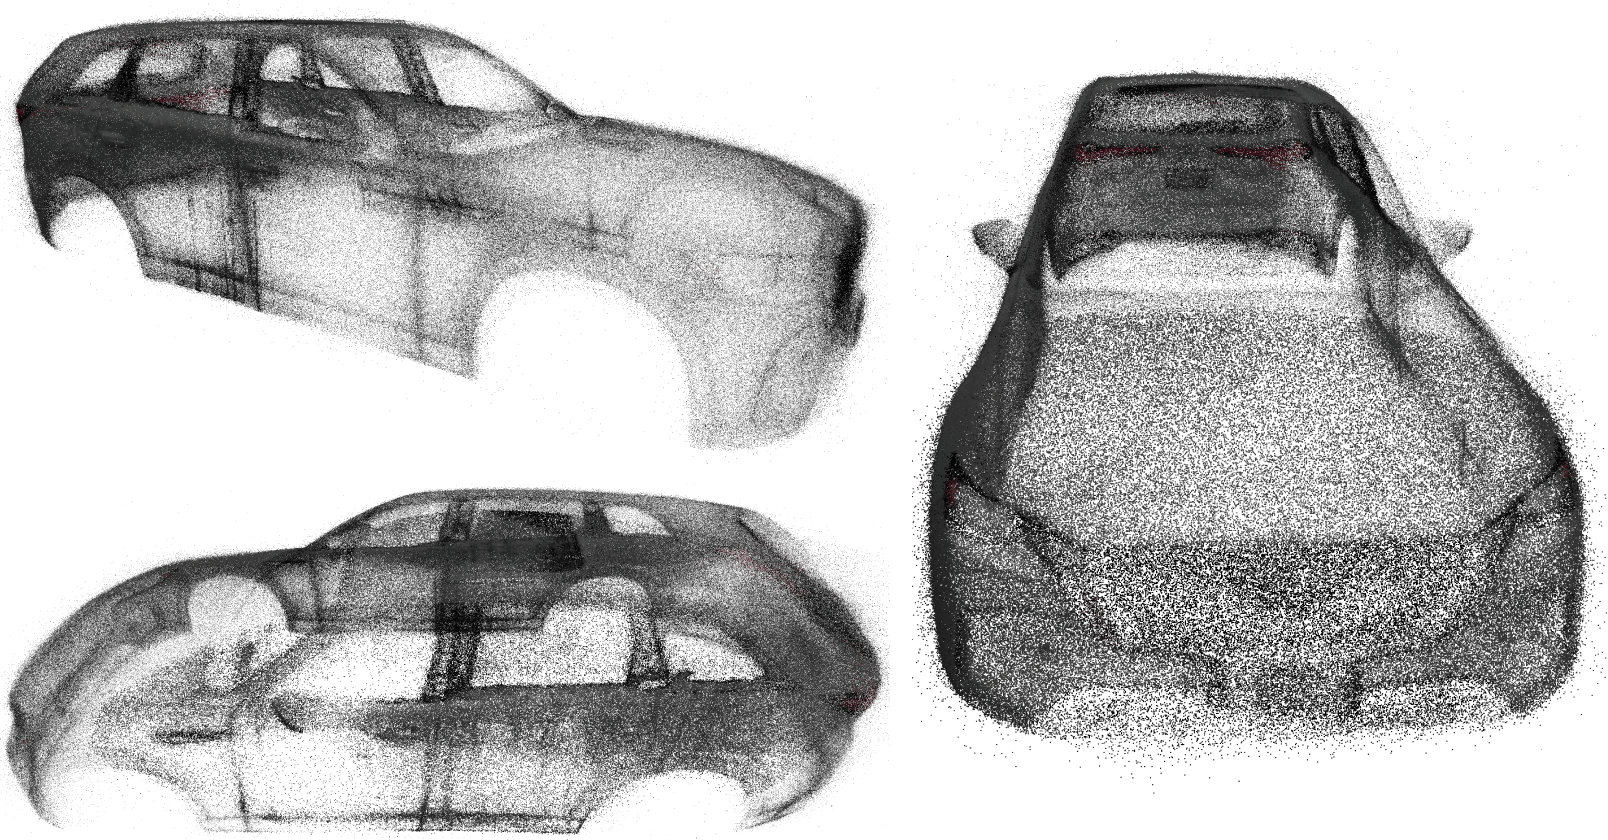
\includegraphics[width=\linewidth]{images_low/sparse_point_clouds_same_vehicle.png}
    \caption{\small Representative successful sparse point cloud produced by the full pipeline, visualized from multiple viewpoints for the same vehicle. The sparse point cloud forms a coherent vehicle shell with limited background structure, providing a stable geometric scaffold for downstream Gaussian Splatting.}
    \label{fig:sparse_point_clouds_ours}
\end{figure}

\begin{figure}[t]
    \centering
    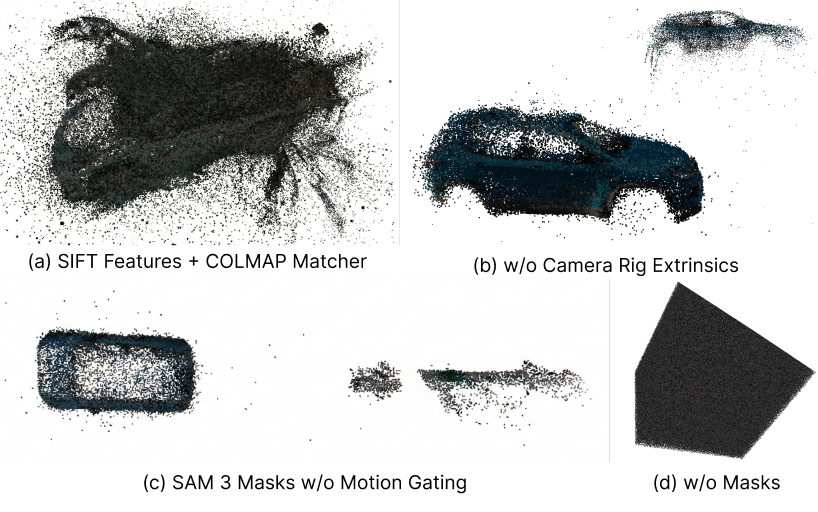
\includegraphics[width=\linewidth]{images_low/sparse_point_cloud_ablations.png}
    \caption{\small Sparse point cloud failure modes from ablations. \textbf{(a) SIFT Features + COLMAP Matcher:} Relying on classical keypoints rather than our mask-guided learned matcher results in massive point cloud fragmentation and noise, as classical methods fail to establish reliable tracks across highly specular automotive clear coats. \textbf{(b) w/o Camera Rig Extrinsics:} Without CAD-derived relative pose priors, the wide-baseline optimization suffers from inter-camera drift, producing fragmented reconstructions. \textbf{(c) SAM 3 Masks w/o Motion Gating:} Relying purely on semantic instance masks without temporal motion gating causes the instance tracking to drift onto parked distractor vehicles in the background when the primary target is partially absent. \textbf{(d) w/o Masks:} Correspondences are dominated by the static dealership environment, producing a background-centric ``room-like'' reconstruction (cube/planes) with little vehicle geometry.}
    \label{fig:sparse_point_cloud_ablations}
\end{figure}
































% \subsection{Gaussian Splatting}
% \label{sec:exp_gs}
% % Rendering Metrics + Qualitative

% % For GS, include PSNR/SSIM on held-out views; focus on qualitative + user-facing “view from all angles” outcomes (interactive render snapshots).


% The rig-aware SfM stage yields a metrically consistent geometric initialization. To synthesize photorealistic, interactive novel views of the vehicle exterior, we transition to dense volumetric rendering. Crucially, we replace the strict rigid-body masks ($\mathcal{M}_{\text{rigid}}$) with complete vehicle rendering masks ($\mathcal{M}_{\text{render}}$) to explicitly reconstruct the rotating wheels while ignoring dealership clutter.

% To quantitatively evaluate view synthesis fidelity, we temporally sample 10\% of the synchronized 4K frames across all 14 cameras as a held-out test set. We evaluate three rendering architectures: (1) Standard 3D-GS, which requires destructively pre-undistorted imagery; (2) 3DGUT, utilizing native fisheye parameters directly on raw frames; and (3) our full pipeline coupling 3DGUT with Markov Chain Monte Carlo (MCMC) densification to escape local minima on highly specular automotive clear coats. 


% \begin{table}[ht]
% % \vspace{-0.15cm}
% \centering
% \caption{Gaussian Splatting ablation study on held-out views. Each column modifies the rendering architecture relative to the full pipeline.}
% \label{tab:gs_ablations}
% \setlength{\tabcolsep}{4pt}
% % \renewcommand{\arraystretch}{1.2}
% % \resizebox{\columnwidth}{!}{
% \begin{tabular}{lccc}
% \hline
% \textbf{Metric} &
% \begin{tabular}[c]{@{}c@{}}\textbf{Standard 3D-GS} \\ \textbf{(Undistorted)}\end{tabular} &
% \begin{tabular}[c]{@{}c@{}}\textbf{3DGUT} \\ \textbf{(Fisheye)}\end{tabular} &
% \begin{tabular}[c]{@{}c@{}}\textbf{3DGUT + MCMC} \\ \textbf{(Full)}\end{tabular} \\
% \hline

% PSNR $\uparrow$ 
% & 0.00 & 0.00 & \textbf{0.00} \\

% \hline
% SSIM $\uparrow$ 
% & 0.00 & 0.0 & \textbf{0.00} \\

% \hline
% LPIPS $\downarrow$ 
% & 0.0 & 0.00 & \textbf{0.0} \\

% \hline
% \end{tabular}
% \end{table}


% As detailed in Table \ref{tab:gs_ablations}, natively modeling lens distortion and employing stochastic densification drastically reduces view-dependent artifacts such as "floaters" and ghosting. The full pipeline yields pristine, inspection-grade 3D assets, enabling remote buyers to seamlessly orbit and evaluate the vehicle free from background distractions.



% \begin{figure}
%     \centering    \includegraphics[width=1\linewidth]{images/ground_truth_vs_gaussian_splat.png}
%     \caption{Ground Truth vs Gaussian Splat (UPDATE FIGURE TO NOT MAKE THE RIGHT REAR PASSENGER WINDOW TRANSPARENT}    \label{fig:ground_truth_vs_gaussian_splat}
% \end{figure}




% \begin{figure}
%     \centering    \includegraphics[width=1\linewidth]{images/Gaussian Splats.png}
%     \caption{Gaussian Splats}    \label{fig:gaussian_splats}
% \end{figure}











\subsection{Gaussian Splatting}
\label{subsec:experiments_gaussian_splatting}

% The rig-aware SfM stage yields a metrically consistent geometric initialization. 
% To synthesize photorealistic, interactive novel views of the vehicle exterior, we transition to dense volumetric rendering. We replace the strict rigid-body masks ($\mathcal{M}_{\text{rigid}}$) with complete vehicle rendering masks ($\mathcal{M}_{\text{render}}$) to explicitly reconstruct the rotating wheels while ignoring dealership clutter. This is an explicit design choice for the customer; moving wheels can appear blurred and may reduce PSNR/SSIM on held-out views, but they produce a perceptually complete, fully reconstructed vehicle silhouette.

We use standard image quality metrics: Peak Signal-to-Noise Ratio (PSNR), Structural Similarity Index (SSIM), and the perceptual Learned Perceptual Image Patch Similarity (LPIPS) metric. We use complete vehicle rendering masks ($\mathcal{M}_{\text{render}}$) to reconstruct the rotating wheels while ignoring dealership clutter. This is an explicit design choice for the customer; moving wheels can appear blurred and may reduce PSNR/SSIM on held-out views, but they produce a perceptually complete, fully reconstructed vehicle silhouette.


We temporally sample 10\% of the 4K frames across all 14 cameras as a held-out test set. Fig.~\ref{fig:ground_truth_vs_gaussian_splat} highlights the strong photometric correlation between the held-out ground truth frames and our rendered outputs. We evaluate three rendering architectures: (1) Standard 3D-GS, which requires undistorted images; (2) 3DGUT, utilizing native fisheye parameters directly on raw frames; and (3) our full pipeline coupling 3DGUT with MCMC densification to escape local minima on specular automotive clear coats. 

\begin{table}[ht]
% \vspace{-0.15cm}
\centering
\caption{\small Gaussian Splatting ablation study on held-out views. Each column modifies the architecture relative to the full pipeline.}
\label{tab:gs_ablations}
\setlength{\tabcolsep}{4pt}
% \renewcommand{\arraystretch}{1.2}
% \resizebox{\columnwidth}{!}{
\begin{tabular}{lccc}
\hline
\textbf{Metric} &
\begin{tabular}[c]{@{}c@{}}\textbf{Standard 3D-GS} \\ \textbf{(Undistorted)}\end{tabular} &
\begin{tabular}[c]{@{}c@{}}\textbf{3DGUT} \\ \textbf{(Fisheye)}\end{tabular} &
\begin{tabular}[c]{@{}c@{}}\textbf{3DGUT + MCMC} \\ \textbf{(Ours)}\end{tabular} \\
\hline

PSNR $\uparrow$ 
& 24.81 & 27.19 & \textbf{28.66} \\

\hline
SSIM $\uparrow$ 
& 0.81 & 0.86 & \textbf{0.89} \\

\hline
LPIPS $\downarrow$ 
& 0.28 & 0.22 & \textbf{0.21} \\

\hline
\end{tabular}
\end{table}

Our pipeline achieves a mean PSNR of $28.66$ dB, a mean SSIM of $0.89$, and a mean LPIPS of $0.21$, indicating that our rendered views are visually and perceptually closer to the real camera images. This demonstrates a clear improvement over 3DGS, which uses undistorted images, indicating that modeling fisheye distortion produces a superior splat (Tab.~\ref{tab:gs_ablations}). The full pipeline yields a high-quality 3D model. This enables remote buyers to seamlessly orbit and evaluate the vehicle from arbitrary viewpoints, completely free from background distractions. 

Training takes $\approx 20-30$ minutes on an RTX A6000 GPU. Efficient training and a high-fidelity 3D model enable us to view the vehicle from different angles, making it practical for production use.

\vspace{-1em}

\begin{figure}[ht]
    \centering
    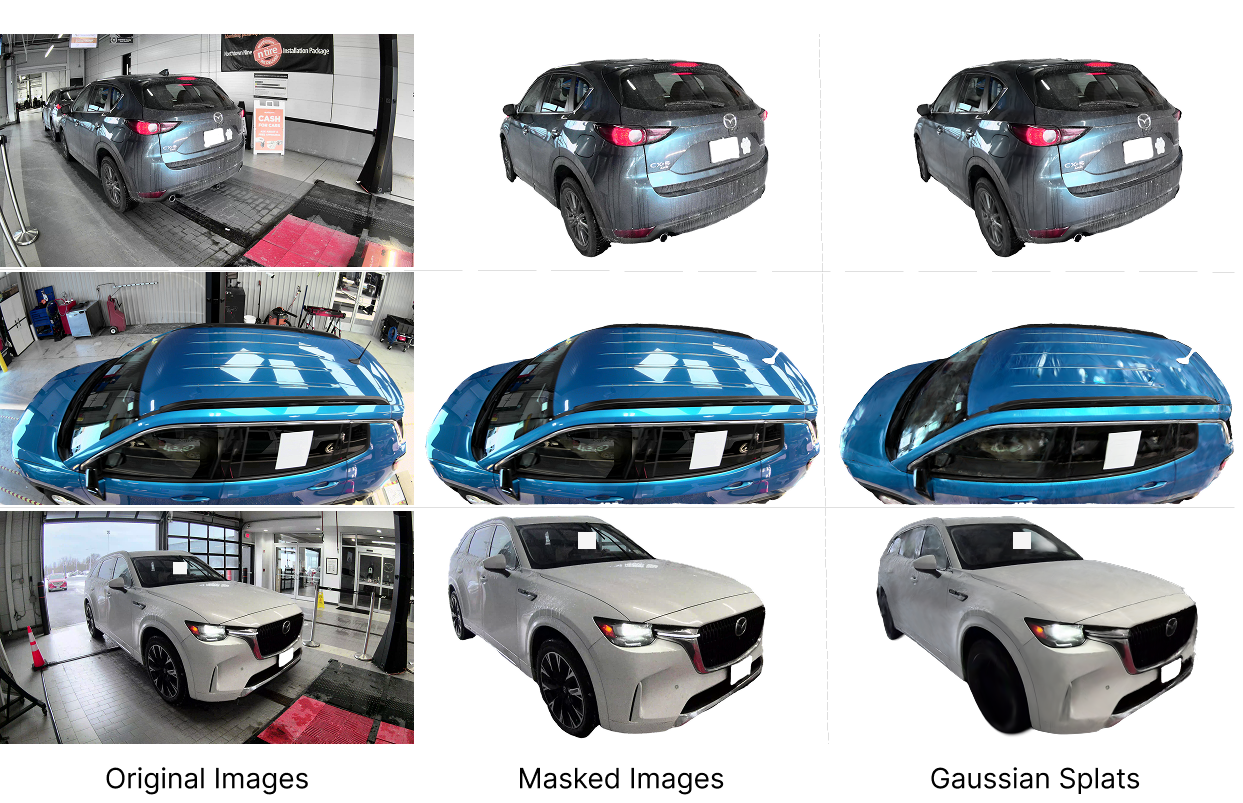
\includegraphics[width=1\linewidth]{images_low/ground_truth_gaussian_splat.png}
    % \caption{\small Ground Truth (left) vs Gaussian Splat (right) (license plate masked for privacy). Our pipeline accurately preserves specular reflections and panel micro-textures on held-out views.}
    \caption{\small End-to-end rendering examples (license plates and driver masked for privacy). \textbf{Left:} Original images captured from the cluttered dealership environment. \textbf{Middle:} Complete vehicle rendering masks ($M^{\text{render}}$) applied to isolate the vehicle and explicitly retain the wheels. \textbf{Right:} 3DGUT Gaussian Splatting renders from the corresponding viewpoints.}
    % \caption{\small End-to-end rendering examples (license plates and driver masked for privacy).\textbf{ Left:} Original images from our camera rig. \textbf{Middle:} Complete vehicle rendering masks ($M^{\text{render}}$) applied to isolate the vehicle during 3DGUT training (wheels included). \textbf{Right:} 3DGUT Gaussian Splatting renders from the corresponding viewpoints.}
    \label{fig:ground_truth_vs_gaussian_splat}
\end{figure}

\vspace{-1em}

% \begin{figure}[ht]
%     \centering
%     \includegraphics[width=1\linewidth]{images_low/ground_truth_vs_gaussian_splat.png}
%     \caption{\small Ground Truth (left) vs Gaussian Splat (right) (license plate masked for privacy). Our pipeline accurately preserves specular reflections and panel micro-textures on held-out views.}
%     \label{fig:ground_truth_vs_gaussian_splat}
% \end{figure}

% \begin{figure}[ht]
%     \centering
%     \includegraphics[width=1\linewidth]{images_low/gaussian_splats.png}
%     \caption{\small Final Gaussian Splats (license plate and driver masked for privacy). The resulting splats provide a visually complete, artifact-free exterior twin suitable for all-angle remote inspection.}
%     \label{fig:gaussian_splats}
% \end{figure}


% \subsection{Gaussian Splatting}
% \label{sec:exp_gs}

% The rig-aware SfM stage yields metrically consistent fisheye poses and a sparse vehicle-centric scaffold, which we use to initialize dense neural rendering. We train a distortion-aware Gaussian Splatting model using 3DGUT \cite{kerbl20233dgs,pan20243dgut} to synthesize photorealistic, interactive novel views of the vehicle exterior. Unlike SfM, which must enforce rigidity, rendering benefits from visual completeness: we therefore replace rigid-body masks ($\mathcal{M}_{\text{rigid}}$, wheels removed) with full vehicle masks ($\mathcal{M}_{\text{render}}$, wheels included). This is an explicit design choice for customer inspection---moving wheels can appear slightly blurred and may reduce PSNR/SSIM on held-out views, but they produce a perceptually complete, fully reconstructed vehicle silhouette.

% \paragraph{Protocol and metrics.}
% We temporally sample $10\%$ of synchronized 4K frames across all 14 cameras as a held-out set. For each held-out image $\mathbf{I}$ and rendered image $\hat{\mathbf{I}}$, metrics are computed over the foreground region $\Omega_M=\{\mathbf{u}\mid M(\mathbf{u})=1\}$:
% \begin{equation}
% \mathrm{MSE}=\frac{1}{|\Omega_M|}\sum_{\mathbf{u}\in\Omega_M}\|\mathbf{I}(\mathbf{u})-\hat{\mathbf{I}}(\mathbf{u})\|_2^2,\quad
% \mathrm{PSNR}=10\log_{10}\!\left(\frac{1}{\mathrm{MSE}}\right),
% \end{equation}
% with SSIM and LPIPS also reported on $\Omega_M$.

% \paragraph{Ablations.}
% We compare three rendering architectures: (i) standard 3D Gaussian Splatting (3DGS) trained on pre-undistorted imagery \cite{kerbl20233dgs}; (ii) 3DGUT, which natively models fisheye distortion via distortion-aware rasterization \cite{pan20243dgut}; and (iii) our full rendering pipeline, which combines 3DGUT with an MCMC densification strategy to improve convergence on highly specular automotive surfaces. Quantitative results are summarized in Table~\ref{tab:gs_ablations}, and qualitative differences are illustrated in Fig.~\ref{fig:gaussian_splats_ablations}.

% \begin{table}[t]
% \centering
% \caption{Gaussian Splatting ablation study on held-out views. Distortion-native rendering and stochastic densification improve view synthesis under wide-FOV optics and specular appearance.}
% \label{tab:gs_ablations}
% \setlength{\tabcolsep}{4pt}
% \begin{tabular}{lccc}
% \hline
% \textbf{Metric} &
% \begin{tabular}[c]{@{}c@{}}\textbf{3DGS} \\ \textbf{(Undistorted)}\end{tabular} &
% \begin{tabular}[c]{@{}c@{}}\textbf{3DGUT} \\ \textbf{(Fisheye)}\end{tabular} &
% \begin{tabular}[c]{@{}c@{}}\textbf{3DGUT + MCMC} \\ \textbf{(Full)}\end{tabular} \\
% \hline
% PSNR $\uparrow$  & 0.00 & 0.00 & \textbf{0.00} \\
% SSIM $\uparrow$  & 0.00 & 0.00 & \textbf{0.00} \\
% LPIPS $\downarrow$ & 0.00 & 0.00 & \textbf{0.00} \\
% \hline
% \end{tabular}
% \end{table}

% \paragraph{Qualitative results.}
% Figure~\ref{fig:ground_truth_vs_gaussian_splat} shows representative held-out comparisons between ground truth and our 3DGUT rendering, where remaining discrepancies are primarily due to view-dependent specularities and residual motion in the wheels. Figure~\ref{fig:gaussian_splats} presents qualitative 3DGUT reconstructions demonstrating all-angle inspection capability (orbiting viewpoints, consistent body geometry, and suppression of dealership clutter). Finally, Fig.~\ref{fig:gaussian_splats_ablations} visualizes failure modes addressed by distortion-native rendering and MCMC densification, including ``floaters'' and ghosting caused by pose noise and specular highlights.

% \paragraph{Implication for deployment.}
% Overall, distortion-aware Gaussian Splatting driven by rig-consistent SfM yields inspection-grade 3D assets suitable for remote vehicle viewing. The ablations confirm that retaining raw fisheye imagery through rendering and using stochastic densification materially improves fidelity in the deployment regime considered in this work.

% \begin{figure}[t]
%     \centering
%     \includegraphics[width=\linewidth]{images/ground_truth_vs_gaussian_splat.png}
%     \caption{Held-out view comparison between a ground-truth frame and our 3DGUT rendering \cite{pan20243dgut}. Minor residual errors are dominated by specular effects and wheel motion.}
%     \label{fig:ground_truth_vs_gaussian_splat}
% \end{figure}

% \begin{figure}[t]
%     \centering
%     \includegraphics[width=\linewidth]{images/Gaussian Splats.png}
%     \caption{Qualitative 3DGUT Gaussian Splatting results enabling all-angle exterior inspection from a single drive-through capture.}
%     \label{fig:gaussian_splats}
% \end{figure}

% \begin{figure}[t]
%     \centering
%     \includegraphics[width=\linewidth]{images/Gaussian Splats Ablations.png}
%     \caption{Qualitative ablations for Gaussian Splatting. Distortion-native rendering (3DGUT) and MCMC densification reduce ghosting and ``floaters'' relative to undistorted 3DGS baselines.}
%     \label{fig:gaussian_splats_ablations}
% \end{figure}

\section{Conclusion}
\label{sec:conclusion}

This paper presented a modular, end-to-end pipeline for high-fidelity 3D reconstruction of vehicle exteriors in active, high-throughput drive-through environments. We addressed the fundamental challenge of dynamic-scene SfM within cluttered dealership settings. Our motion-gated semantic isolation strategy, coupled with the explicit subtraction of non-rigid wheels, ensured mathematical compliance with epipolar geometry, while the use of CAD-derived rig priors eliminated scale drift across wide physical baselines. Furthermore, our distortion-native learned matching and MCMC-driven 3DGUT successfully navigated the complexities of extreme wide-angle lenses and highly reflective automotive surfaces. Evaluations on real-world captures demonstrate that our system provides inspection-grade 3D assets without the need for controlled studio infrastructure. Future work will focus on integrating automated anomaly detection directly into the 3DGS volume to streamline the identification of exterior defects.

% This paper presents a deployable, end-to-end pipeline for 3D vehicle exterior reconstruction in unconstrained dealership drive-through environments. To resolve the fundamental dynamic-scene ambiguity against static background clutter, we couple SAM 3 with motion-gating logic to isolate the vehicle. Crucially, we explicitly enforce SfM rigidity by subtracting non-rigid wheel rotations:
% \begin{equation}
%     M^{\text{rigid}}_{c,t} \;=\; M_{c,t} \wedge \neg W_{c,t}
% \end{equation}
% Executing mask-aware RoMA v2 matching directly on raw fisheye camera images and constraining the global bundle adjustment with CAD-derived rig priors successfully eliminates scale drift. Natively modeling this distortion within the 3DGUT Gaussian Splatting architecture via stochastic densification yields inspection-grade 3D assets with state-of-the-art photometric fidelity. 


\bibliographystyle{IEEEtran}
\bibliography{references}






\end{document}

































%%%%%%%%%%%%%%%%%%%%%%%%%%%%%%%%%%%%%%%%%%%%%%%%%%%%%%%%%%%%%%%%%%%%%%%%%%%%%%%%
% \section{INTRODUCTION}

% This template provides authors with most of the formatting specifications needed for preparing electronic versions of their papers. All standard paper components have been specified for three reasons: (1) ease of use when formatting individual papers, (2) automatic compliance to electronic requirements that facilitate the concurrent or later production of electronic products, and (3) conformity of style throughout a conference proceedings. Margins, column widths, line spacing, and type styles are built-in; examples of the type styles are provided throughout this document and are identified in italic type, within parentheses, following the example. Some components, such as multi-leveled equations, graphics, and tables are not prescribed, although the various table text styles are provided. The formatter will need to create these components, incorporating the applicable criteria that follow.

% \section{PROCEDURE FOR PAPER SUBMISSION}

% \subsection{Selecting a Template (Heading 2)}

% First, confirm that you have the correct template for your paper size. This template has been tailored for output on the US-letter paper size. 
% It may be used for A4 paper size if the paper size setting is suitably modified.

% \subsection{Maintaining the Integrity of the Specifications}

% The template is used to format your paper and style the text. All margins, column widths, line spaces, and text fonts are prescribed; please do not alter them. You may note peculiarities. For example, the head margin in this template measures proportionately more than is customary. This measurement and others are deliberate, using specifications that anticipate your paper as one part of the entire proceedings, and not as an independent document. Please do not revise any of the current designations

% \section{MATH}

% Before you begin to format your paper, first write and save the content as a separate text file. Keep your text and graphic files separate until after the text has been formatted and styled. Do not use hard tabs, and limit use of hard returns to only one return at the end of a paragraph. Do not add any kind of pagination anywhere in the paper. Do not number text heads-the template will do that for you.

% Finally, complete content and organizational editing before formatting. Please take note of the following items when proofreading spelling and grammar:

% \subsection{Abbreviations and Acronyms} Define abbreviations and acronyms the first time they are used in the text, even after they have been defined in the abstract. Abbreviations such as IEEE, SI, MKS, CGS, sc, dc, and rms do not have to be defined. Do not use abbreviations in the title or heads unless they are unavoidable.

% \subsection{Units}

% \begin{itemize}

% \item Use either SI (MKS) or CGS as primary units. (SI units are encouraged.) English units may be used as secondary units (in parentheses). An exception would be the use of English units as identifiers in trade, such as Ò3.5-inch disk driveÓ.
% \item Avoid combining SI and CGS units, such as current in amperes and magnetic field in oersteds. This often leads to confusion because equations do not balance dimensionally. If you must use mixed units, clearly state the units for each quantity that you use in an equation.
% \item Do not mix complete spellings and abbreviations of units: ÒWb/m2Ó or Òwebers per square meterÓ, not Òwebers/m2Ó.  Spell out units when they appear in text: Ò. . . a few henriesÓ, not Ò. . . a few HÓ.
% \item Use a zero before decimal points: Ò0.25Ó, not Ò.25Ó. Use Òcm3Ó, not ÒccÓ. (bullet list)

% \end{itemize}


% \subsection{Equations}

% The equations are an exception to the prescribed specifications of this template. You will need to determine whether or not your equation should be typed using either the Times New Roman or the Symbol font (please no other font). To create multileveled equations, it may be necessary to treat the equation as a graphic and insert it into the text after your paper is styled. Number equations consecutively. Equation numbers, within parentheses, are to position flush right, as in (1), using a right tab stop. To make your equations more compact, you may use the solidus ( / ), the exp function, or appropriate exponents. Italicize Roman symbols for quantities and variables, but not Greek symbols. Use a long dash rather than a hyphen for a minus sign. Punctuate equations with commas or periods when they are part of a sentence, as in

% $$
% \alpha + \beta = \chi \eqno{(1)}
% $$

% Note that the equation is centered using a center tab stop. Be sure that the symbols in your equation have been defined before or immediately following the equation. Use Ò(1)Ó, not ÒEq. (1)Ó or Òequation (1)Ó, except at the beginning of a sentence: ÒEquation (1) is . . .Ó

% \subsection{Some Common Mistakes}
% \begin{itemize}


% \item The word ÒdataÓ is plural, not singular.
% \item The subscript for the permeability of vacuum ?0, and other common scientific constants, is zero with subscript formatting, not a lowercase letter ÒoÓ.
% \item In American English, commas, semi-/colons, periods, question and exclamation marks are located within quotation marks only when a complete thought or name is cited, such as a title or full quotation. When quotation marks are used, instead of a bold or italic typeface, to highlight a word or phrase, punctuation should appear outside of the quotation marks. A parenthetical phrase or statement at the end of a sentence is punctuated outside of the closing parenthesis (like this). (A parenthetical sentence is punctuated within the parentheses.)
% \item A graph within a graph is an ÒinsetÓ, not an ÒinsertÓ. The word alternatively is preferred to the word ÒalternatelyÓ (unless you really mean something that alternates).
% \item Do not use the word ÒessentiallyÓ to mean ÒapproximatelyÓ or ÒeffectivelyÓ.
% \item In your paper title, if the words Òthat usesÓ can accurately replace the word ÒusingÓ, capitalize the ÒuÓ; if not, keep using lower-cased.
% \item Be aware of the different meanings of the homophones ÒaffectÓ and ÒeffectÓ, ÒcomplementÓ and ÒcomplimentÓ, ÒdiscreetÓ and ÒdiscreteÓ, ÒprincipalÓ and ÒprincipleÓ.
% \item Do not confuse ÒimplyÓ and ÒinferÓ.
% \item The prefix ÒnonÓ is not a word; it should be joined to the word it modifies, usually without a hyphen.
% \item There is no period after the ÒetÓ in the Latin abbreviation Òet al.Ó.
% \item The abbreviation Òi.e.Ó means Òthat isÓ, and the abbreviation Òe.g.Ó means Òfor exampleÓ.

% \end{itemize}


% \section{USING THE TEMPLATE}

% Use this sample document as your LaTeX source file to create your document. Save this file as {\bf root.tex}. You have to make sure to use the cls file that came with this distribution. If you use a different style file, you cannot expect to get required margins. Note also that when you are creating your out PDF file, the source file is only part of the equation. {\it Your \TeX\ $\rightarrow$ PDF filter determines the output file size. Even if you make all the specifications to output a letter file in the source - if your filter is set to produce A4, you will only get A4 output. }

% It is impossible to account for all possible situation, one would encounter using \TeX. If you are using multiple \TeX\ files you must make sure that the ``MAIN`` source file is called root.tex - this is particularly important if your conference is using PaperPlaza's built in \TeX\ to PDF conversion tool.

% \subsection{Headings, etc}

% Text heads organize the topics on a relational, hierarchical basis. For example, the paper title is the primary text head because all subsequent material relates and elaborates on this one topic. If there are two or more sub-topics, the next level head (uppercase Roman numerals) should be used and, conversely, if there are not at least two sub-topics, then no subheads should be introduced. Styles named ÒHeading 1Ó, ÒHeading 2Ó, ÒHeading 3Ó, and ÒHeading 4Ó are prescribed.

% \subsection{Figures and Tables}

% Positioning Figures and Tables: Place figures and tables at the top and bottom of columns. Avoid placing them in the middle of columns. Large figures and tables may span across both columns. Figure captions should be below the figures; table heads should appear above the tables. Insert figures and tables after they are cited in the text. Use the abbreviation ÒFig. 1Ó, even at the beginning of a sentence.

% \begin{table}[h]
% \caption{An Example of a Table}
% \label{table_example}
% \begin{center}
% \begin{tabular}{|c||c|}
% \hline
% One & Two\\
% \hline
% Three & Four\\
% \hline
% \end{tabular}
% \end{center}
% \end{table}


%    \begin{figure}[thpb]
%       \centering
%       \framebox{\parbox{3in}{We suggest that you use a text box to insert a graphic (which is ideally a 300 dpi TIFF or EPS file, with all fonts embedded) because, in an document, this method is somewhat more stable than directly inserting a picture.
% }}
%       %\includegraphics[scale=1.0]{figurefile}
%       \caption{Inductance of oscillation winding on amorphous
%        magnetic core versus DC bias magnetic field}
%       \label{figurelabel}
%    \end{figure}
   

% Figure Labels: Use 8 point Times New Roman for Figure labels. Use words rather than symbols or abbreviations when writing Figure axis labels to avoid confusing the reader. As an example, write the quantity ÒMagnetizationÓ, or ÒMagnetization, MÓ, not just ÒMÓ. If including units in the label, present them within parentheses. Do not label axes only with units. In the example, write ÒMagnetization (A/m)Ó or ÒMagnetization {A[m(1)]}Ó, not just ÒA/mÓ. Do not label axes with a ratio of quantities and units. For example, write ÒTemperature (K)Ó, not ÒTemperature/K.Ó

% \section{CONCLUSIONS}

% A conclusion section is not required. Although a conclusion may review the main points of the paper, do not replicate the abstract as the conclusion. A conclusion might elaborate on the importance of the work or suggest applications and extensions. 

% \addtolength{\textheight}{-12cm}   % This command serves to balance the column lengths
%                                   % on the last page of the document manually. It shortens
%                                   % the textheight of the last page by a suitable amount.
%                                   % This command does not take effect until the next page
%                                   % so it should come on the page before the last. Make
%                                   % sure that you do not shorten the textheight too much.

% %%%%%%%%%%%%%%%%%%%%%%%%%%%%%%%%%%%%%%%%%%%%%%%%%%%%%%%%%%%%%%%%%%%%%%%%%%%%%%%%



% %%%%%%%%%%%%%%%%%%%%%%%%%%%%%%%%%%%%%%%%%%%%%%%%%%%%%%%%%%%%%%%%%%%%%%%%%%%%%%%%



% %%%%%%%%%%%%%%%%%%%%%%%%%%%%%%%%%%%%%%%%%%%%%%%%%%%%%%%%%%%%%%%%%%%%%%%%%%%%%%%%
% \section*{APPENDIX}

% Appendixes should appear before the acknowledgment.

% \section*{ACKNOWLEDGMENT}

% The preferred spelling of the word ÒacknowledgmentÓ in America is without an ÒeÓ after the ÒgÓ. Avoid the stilted expression, ÒOne of us (R. B. G.) thanks . . .Ó  Instead, try ÒR. B. G. thanksÓ. Put sponsor acknowledgments in the unnumbered footnote on the first page.



% %%%%%%%%%%%%%%%%%%%%%%%%%%%%%%%%%%%%%%%%%%%%%%%%%%%%%%%%%%%%%%%%%%%%%%%%%%%%%%%%

% References are important to the reader; therefore, each citation must be complete and correct. If at all possible, references should be commonly available publications.



% \begin{thebibliography}{99}

% \bibitem{c1} G. O. Young, ÒSynthetic structure of industrial plastics (Book style with paper title and editor),Ó 	in Plastics, 2nd ed. vol. 3, J. Peters, Ed.  New York: McGraw-Hill, 1964, pp. 15Ð64.
% \bibitem{c2} W.-K. Chen, Linear Networks and Systems (Book style).	Belmont, CA: Wadsworth, 1993, pp. 123Ð135.
% \bibitem{c3} H. Poor, An Introduction to Signal Detection and Estimation.   New York: Springer-Verlag, 1985, ch. 4.
% \bibitem{c4} B. Smith, ÒAn approach to graphs of linear forms (Unpublished work style),Ó unpublished.
% \bibitem{c5} E. H. Miller, ÒA note on reflector arrays (Periodical styleÑAccepted for publication),Ó IEEE Trans. Antennas Propagat., to be publised.
% \bibitem{c6} J. Wang, ÒFundamentals of erbium-doped fiber amplifiers arrays (Periodical styleÑSubmitted for publication),Ó IEEE J. Quantum Electron., submitted for publication.
% \bibitem{c7} C. J. Kaufman, Rocky Mountain Research Lab., Boulder, CO, private communication, May 1995.
% \bibitem{c8} Y. Yorozu, M. Hirano, K. Oka, and Y. Tagawa, ÒElectron spectroscopy studies on magneto-optical media and plastic substrate interfaces(Translation Journals style),Ó IEEE Transl. J. Magn.Jpn., vol. 2, Aug. 1987, pp. 740Ð741 [Dig. 9th Annu. Conf. Magnetics Japan, 1982, p. 301].
% \bibitem{c9} M. Young, The Techincal Writers Handbook.  Mill Valley, CA: University Science, 1989.
% \bibitem{c10} J. U. Duncombe, ÒInfrared navigationÑPart I: An assessment of feasibility (Periodical style),Ó IEEE Trans. Electron Devices, vol. ED-11, pp. 34Ð39, Jan. 1959.
% \bibitem{c11} S. Chen, B. Mulgrew, and P. M. Grant, ÒA clustering technique for digital communications channel equalization using radial basis function networks,Ó IEEE Trans. Neural Networks, vol. 4, pp. 570Ð578, July 1993.
% \bibitem{c12} R. W. Lucky, ÒAutomatic equalization for digital communication,Ó Bell Syst. Tech. J., vol. 44, no. 4, pp. 547Ð588, Apr. 1965.
% \bibitem{c13} S. P. Bingulac, ÒOn the compatibility of adaptive controllers (Published Conference Proceedings style),Ó in Proc. 4th Annu. Allerton Conf. Circuits and Systems Theory, New York, 1994, pp. 8Ð16.
% \bibitem{c14} G. R. Faulhaber, ÒDesign of service systems with priority reservation,Ó in Conf. Rec. 1995 IEEE Int. Conf. Communications, pp. 3Ð8.
% \bibitem{c15} W. D. Doyle, ÒMagnetization reversal in films with biaxial anisotropy,Ó in 1987 Proc. INTERMAG Conf., pp. 2.2-1Ð2.2-6.
% \bibitem{c16} G. W. Juette and L. E. Zeffanella, ÒRadio noise currents n short sections on bundle conductors (Presented Conference Paper style),Ó presented at the IEEE Summer power Meeting, Dallas, TX, June 22Ð27, 1990, Paper 90 SM 690-0 PWRS.
% \bibitem{c17} J. G. Kreifeldt, ÒAn analysis of surface-detected EMG as an amplitude-modulated noise,Ó presented at the 1989 Int. Conf. Medicine and Biological Engineering, Chicago, IL.
% \bibitem{c18} J. Williams, ÒNarrow-band analyzer (Thesis or Dissertation style),Ó Ph.D. dissertation, Dept. Elect. Eng., Harvard Univ., Cambridge, MA, 1993. 
% \bibitem{c19} N. Kawasaki, ÒParametric study of thermal and chemical nonequilibrium nozzle flow,Ó M.S. thesis, Dept. Electron. Eng., Osaka Univ., Osaka, Japan, 1993.
% \bibitem{c20} J. P. Wilkinson, ÒNonlinear resonant circuit devices (Patent style),Ó U.S. Patent 3 624 12, July 16, 1990. 






% \end{thebibliography}




